%%%%%%%%%%%%%%%%%
% W tagging
%%%%%%%%%%%%%%%%%

One of the main highlights of the razor boost analysis is the tagging of boosted $\W$ bosons in
order to access a signal dominated phase space. 
$\W$ bosons either decay to two quarks, or to a lepton and a neutrino. The razor boost analysis is
an all-hadronic analysis, which means we do not explicitely consider the leptonic decays. 
$\W$ bosons with low to moderate transverse momentum will thus result in two jets, correponding to
the two clusters of particles resulting from the hadronization of the two quarks. 
As the $\pt$ of the $\W$ boson increases, the separation between the two resulting jets decreases.
For high enough momentum, the two jets can no longer be fully resolved with the usual jet
definitions, and will be reconstructed as a single jet. This turnover in efficiency between the
resolved and merged case is illustrated in Fig.~\ref{fig:boost_wtag_ca8eff}.
Depending on the requirements on the jet multiplicity, losing a jet can result in a loss of signal
efficiency. We can, however, also use this effect to our advantage, namely to increase the
signal-to-background ratio by requiring the presence of one of these \textit{merged} jets. 
This, in turn, allows us to relax the jet multiplicity requirements. 

\begin{figure}
  \centering
  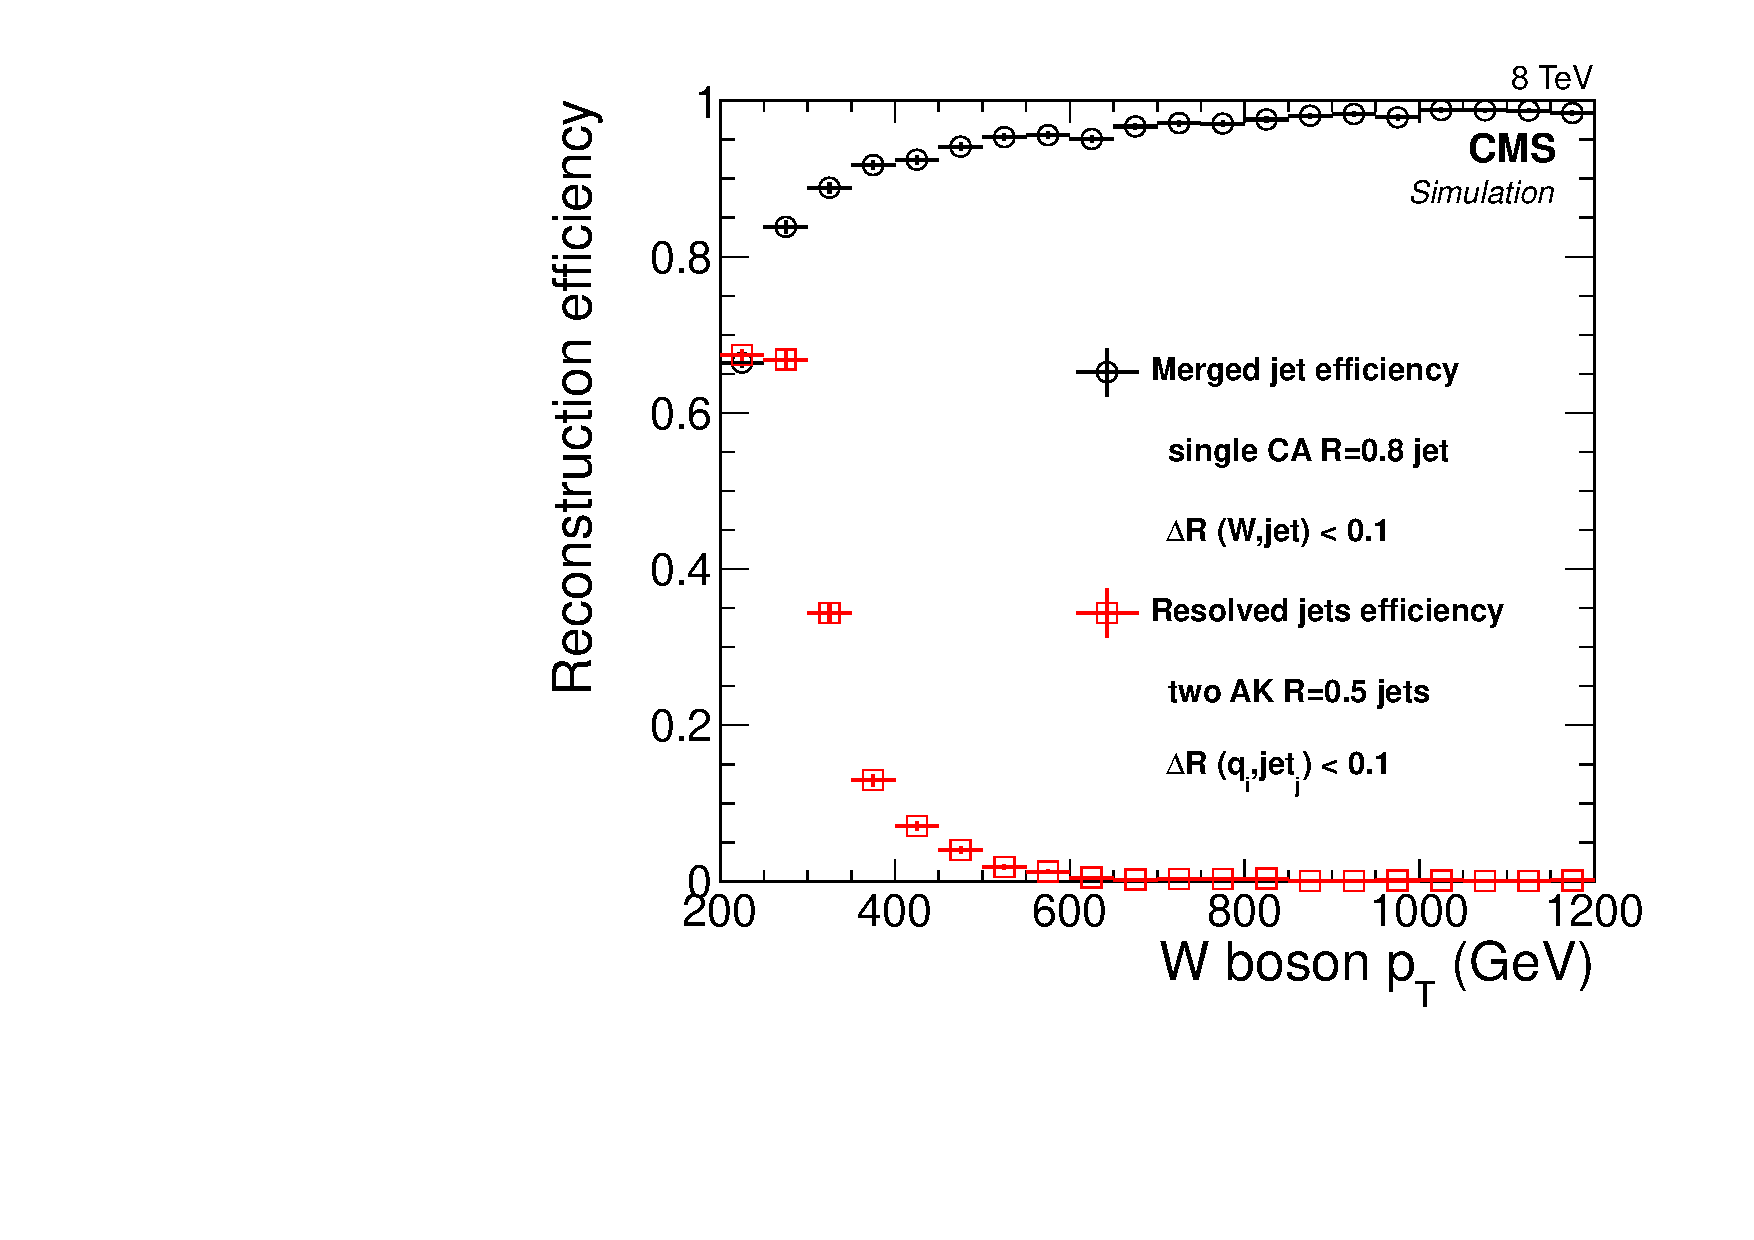
\includegraphics[width=0.7\textwidth]{figures/razor_wtag/ca8effVsPt}
  \caption{Efficiency to reconstruct a CA8 jet within $\Delta R<0.1$ of a generated $\W$ boson, and
the efficiency to reconstruct two AK5 jets within $\Delta R<0.1$ of the generated quarks from
longitudinally polarized $\W$ bosons, as a function of the $\pt$ of the $\W$
boson~\cite{Khachatryan:2014vla}. The loss in efficiency for the resolved case is clearly visible
for high $\pt$ $\W$ bosons. 
  \label{fig:boost_wtag_ca8eff}}
\end{figure}

The merged jet can be distinguished from other jets by its jet substructure, as illustrated in
Fig.~\ref{fig:boost_wtag_cartoon}. Jets originating from a $\W$ boson should have a two-prong
structure, whereas a quark/gluon-initiated jet is not expected to have this structure. 
In recent years, jet substructure techniques have seen very active developments, and many different
options are on the market~\cite{}. For the razor boost analysis we will use the CMS recommendation
in terms of which techniques to use~\cite{CMS-PAS-JME-13-006,Khachatryan:2014vla}. We will employ
\textit{jet pruning} and a set of variables called \textit{N-subjettiness}. On top of these jet
substructure techniques we will also use the jet mass variable to distinguish $\W$-initiated jets
from quark/gluon-initiated jets. 
The following subsections will go through the different parts of the
$\W$ tagging definition, providing a more detailed explanation for each. 
% TODO find jet substructure references

\begin{figure}
  \centering
  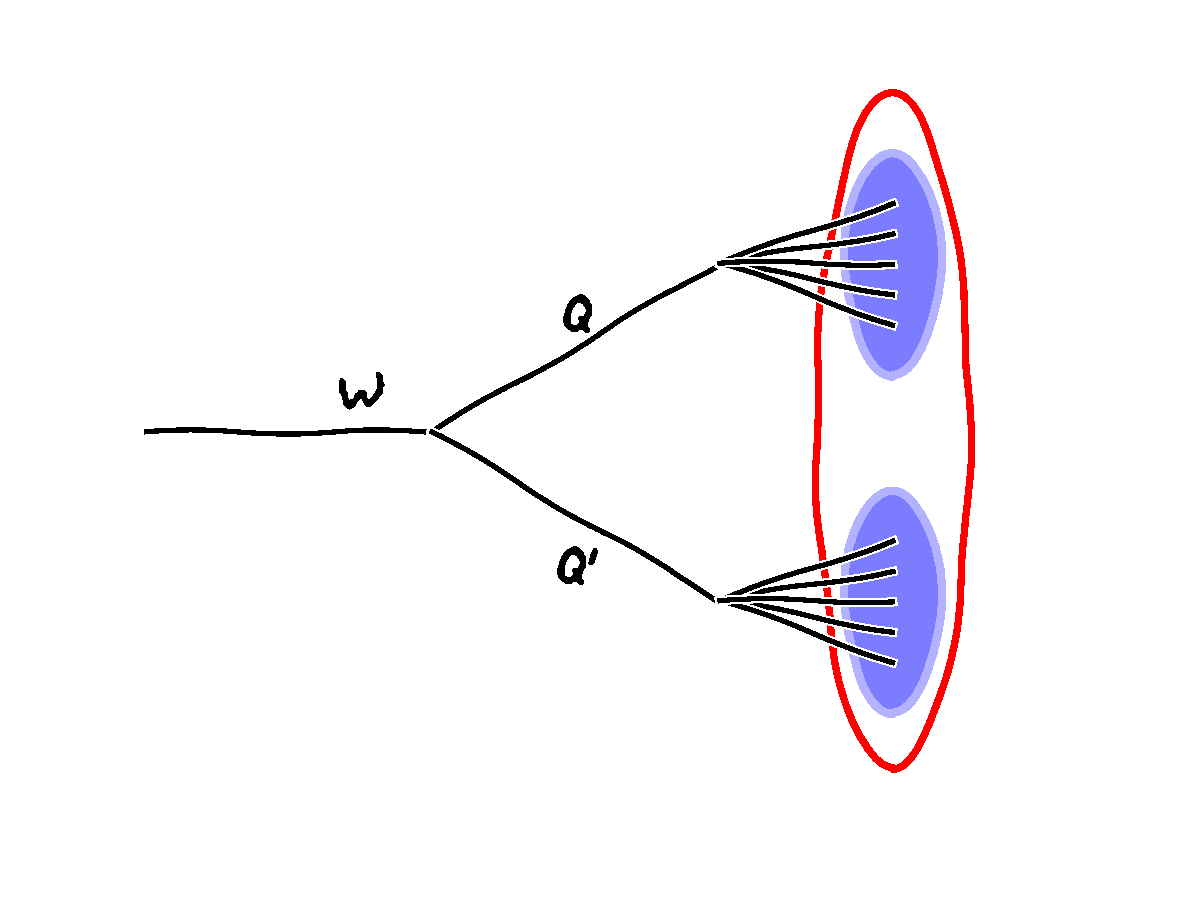
\includegraphics[width=0.48\textwidth]{figures/razor_wtag/W_subjets}
  ~
  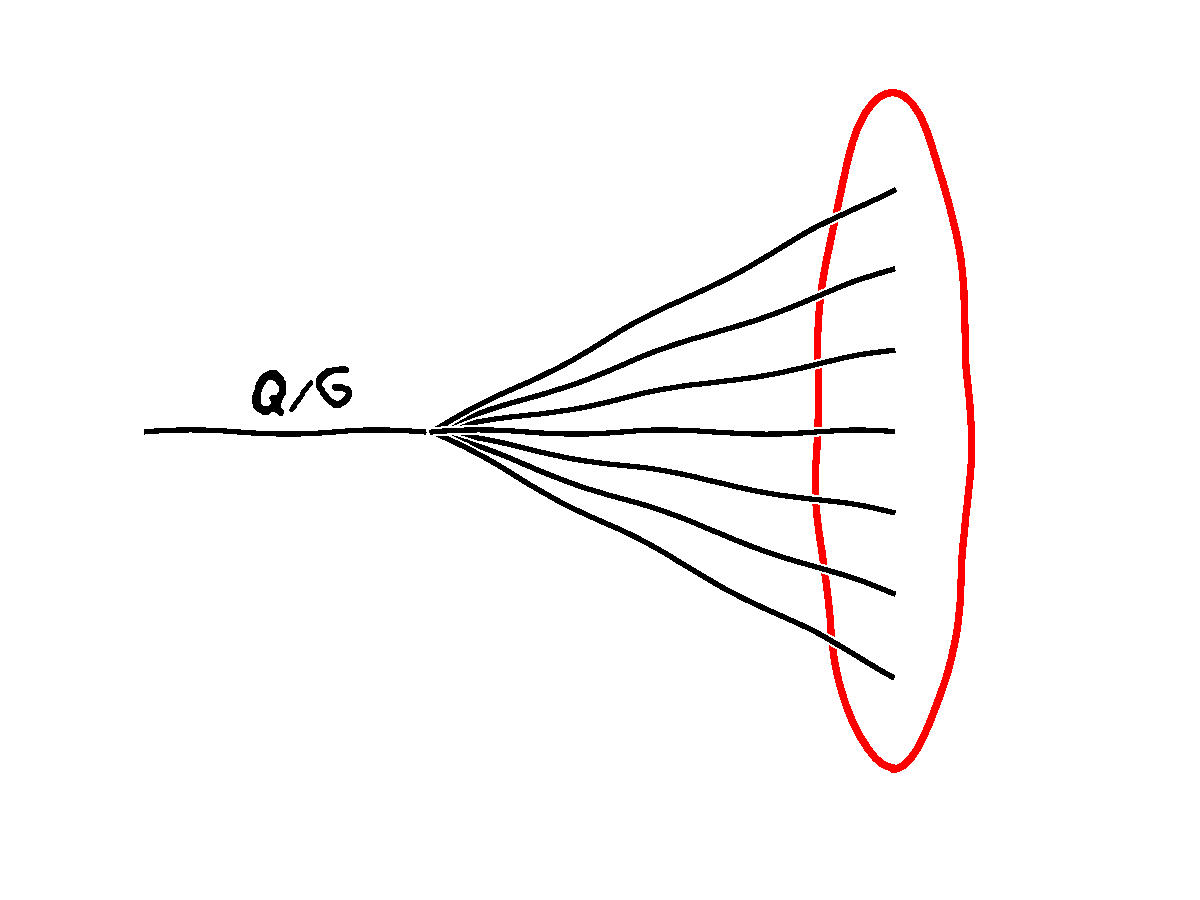
\includegraphics[width=0.48\textwidth]{figures/razor_wtag/qg_jets}
  \caption{The jet substructure of a $\W$-initiated jet differs from a quark/gluon-initiated jet.
  \label{fig:boost_wtag_cartoon}}
\end{figure}

%%%%%%%%%%%%%%%%%%%%%%%%%%%%%%%%%%%%%%%%%%%%%%%%%%%%%%%%%%%%%%%%%%%%%%%%%%%%%%%%%%%%%%%%%%%%%%%%%%%%

\subsection{Jet algorithm}

In order to identify boosted $\W$ bosons,  we will use a different jet clustering algorithm
than what is used for the standard jet definition (see Section~\ref{sec:object_jets}). 
Jets will be clustered with \textsc{FastJet 3.0.1.}~\cite{Cacciari:2011ma}, from the PF candidates,
using the Cambridge-Aachen algorithm~\cite{Dokshitzer:1997in} with a size parameter of 0.8.
Henceforth, we will call these jets \textit{CA8} jets. 

%\begin{quote}
\begin{cajet} \theoremstyle{definition}
The Cambridge-Aachen (CA) jet algorithm is a sequental recombination algorithm that uses the
distance measure $d_{ij}$ between two constituents $i$ and $j$,
\begin{equation}
d_{ij} = \frac{\Delta R_{ij}^2}{R^2}, \label{eq:CA_distance}
\end{equation}
with $R$ the size parameter of the resulting jets, and $\Delta R_{ij}^2 = (y_i - y_j)^2 + (\phi_i -
\phi_j)^2$ where $y, \phi$ are the rapidity and azimuthal angle. The rapidity is given in terms of
energy and longitudinal momentum as
\begin{equation}
  y = \frac{1}{2} \ln{\frac{ E + p_z }{ E - p_z }} .
\end{equation}
The distance between constituent $i$ and the beam is given by $d_{iB} = 1$.
As is clear from the above, these distance measures only use angular information, unlike for the
$k_T$ and anti-$k_T$ algorithms, which use a $\pt$-weighted distance. 

The jet algorithm starts by computing the minimum distance $d_{ij}$, across all $i,j$. If $\min
d_{ij} < d_{iB}$, then we combine constituents $i$ and $j$ into a new constituent whose
four-momentum is the sum of the four-momenta of $i$ and $j$, and repeat the process. Otherwise, we
call $i$ a jet and remove it from the list of constituents to be clustered. Again, the process is
repeated with the remaining constituents, until none remain.
\end{cajet}
%\end{quote}

Jet energy corrections for these CA8 jets are derived from the standard anti-$k_\textrm{T}$ jets
with size parameter $R=0.7$. Simulations show that the corrections are valid for CA8 jets and
have an additional uncertainty no greater than 2\%.  
% TODO find reference for this (some CMS study..)

%We require the CA8 jet mass to lie within the $\W$ boson mass range $70 < m_{jet} < 100$~\GeV
%and call such jets ``mass-tagged" ($Y$).  

%Subjets are obtained by
% undoing or reversing the last step of the clustering algorithm.  



%%%%%%%%%%%%%%%%%%%%%%%%%%%%%%%%%%%%%%%%%%%%%%%%%%%%%%%%%%%%%%%%%%%%%%%%%%%%%%%%%%%%%%%%%%%%%%%%%%%%

\subsection{Jet pruning}

Jet pruning~\cite{Ellis:2009su,Ellis:2009me} is a particular kind of jet grooming. Jet grooming
techniques are designed to reduce the impact of contributions from the underlying event (UE), pileup
(PU), and low-\pt gluon radiation. These kinds of contributions to jets are typically soft and
diffuse, and increase the jet energy proportional to the jet area. Grooming techniques reduce the
jet area without affecting the core components. This means that the resulting jets are less
sensitive to these soft contributions, but still reflect the kinematics of the original, hard
process.


During jet pruning the constituents of the jet are reclustered through the CA algorithm, using the
same distance parameter as used for the original jets (here $R=0.8$), but with additional conditions
beyond those of the standard algorithm.
In particular, the softer and larger-angle of the two particles $i$ and $j$ to be merged is removed
when the following conditions are satisfied:
\begin{align}
  z_{ij} &= \frac{\min( \pt^i , \pt^j )}{\pt^i + \pt^j} < z_{\textrm{cut}}, \\
  \Delta R_{ij} &> D_{\textrm{cut}} \equiv \alpha \frac{m_J}{\pt} ,
\end{align}
where $m_J$ and $\pt$ are the mass and transverse momentum of the originally-clustered jet, and
$z_\textrm{cut}$ and $\alpha$ are parameters of the algorithm, chosen to be 0.1 and 0.5,
respectively~\cite{Chatrchyan:2013vbb}. 

The resulting pruned jet is used as further input to our $\W$ tagger. For the $\W$ decay products
to be collimated, we need a large transverse momentum. We will therefore require that the pruned
jets have $\pt > 200\GeV$. 
Because of the reduction of the effect of UE and PU, the jet mass variable as computed from the
constituents of the jet after jet pruning has a much better behavior than if it was computed from
the unpruned jets, see Fig.~\ref{fig:wtag_jet_pruning}. Jet pruning shifts the jet mass of QCD jets
to smaller values, while maintaining the jet mass for $\W$ jets close to the $\W$ mass.

We will make the requirement that the pruned jet mass is consistent with the $\W$ boson mass,
\begin{equation}
  70 < m_{\textrm{pruned jet}} < 100 \GeV .
\end{equation}
Here, we have deviated from the standard interval starting at 60\GeV, as we found that for our
kinematical region and signal topology we achieve better signal to background discrimination when
increasing the lower cut value to 70\GeV. 
%This provides good boosted $\W$ jet to quark/gluon jet discrimination. 

\begin{figure}
  \centering
  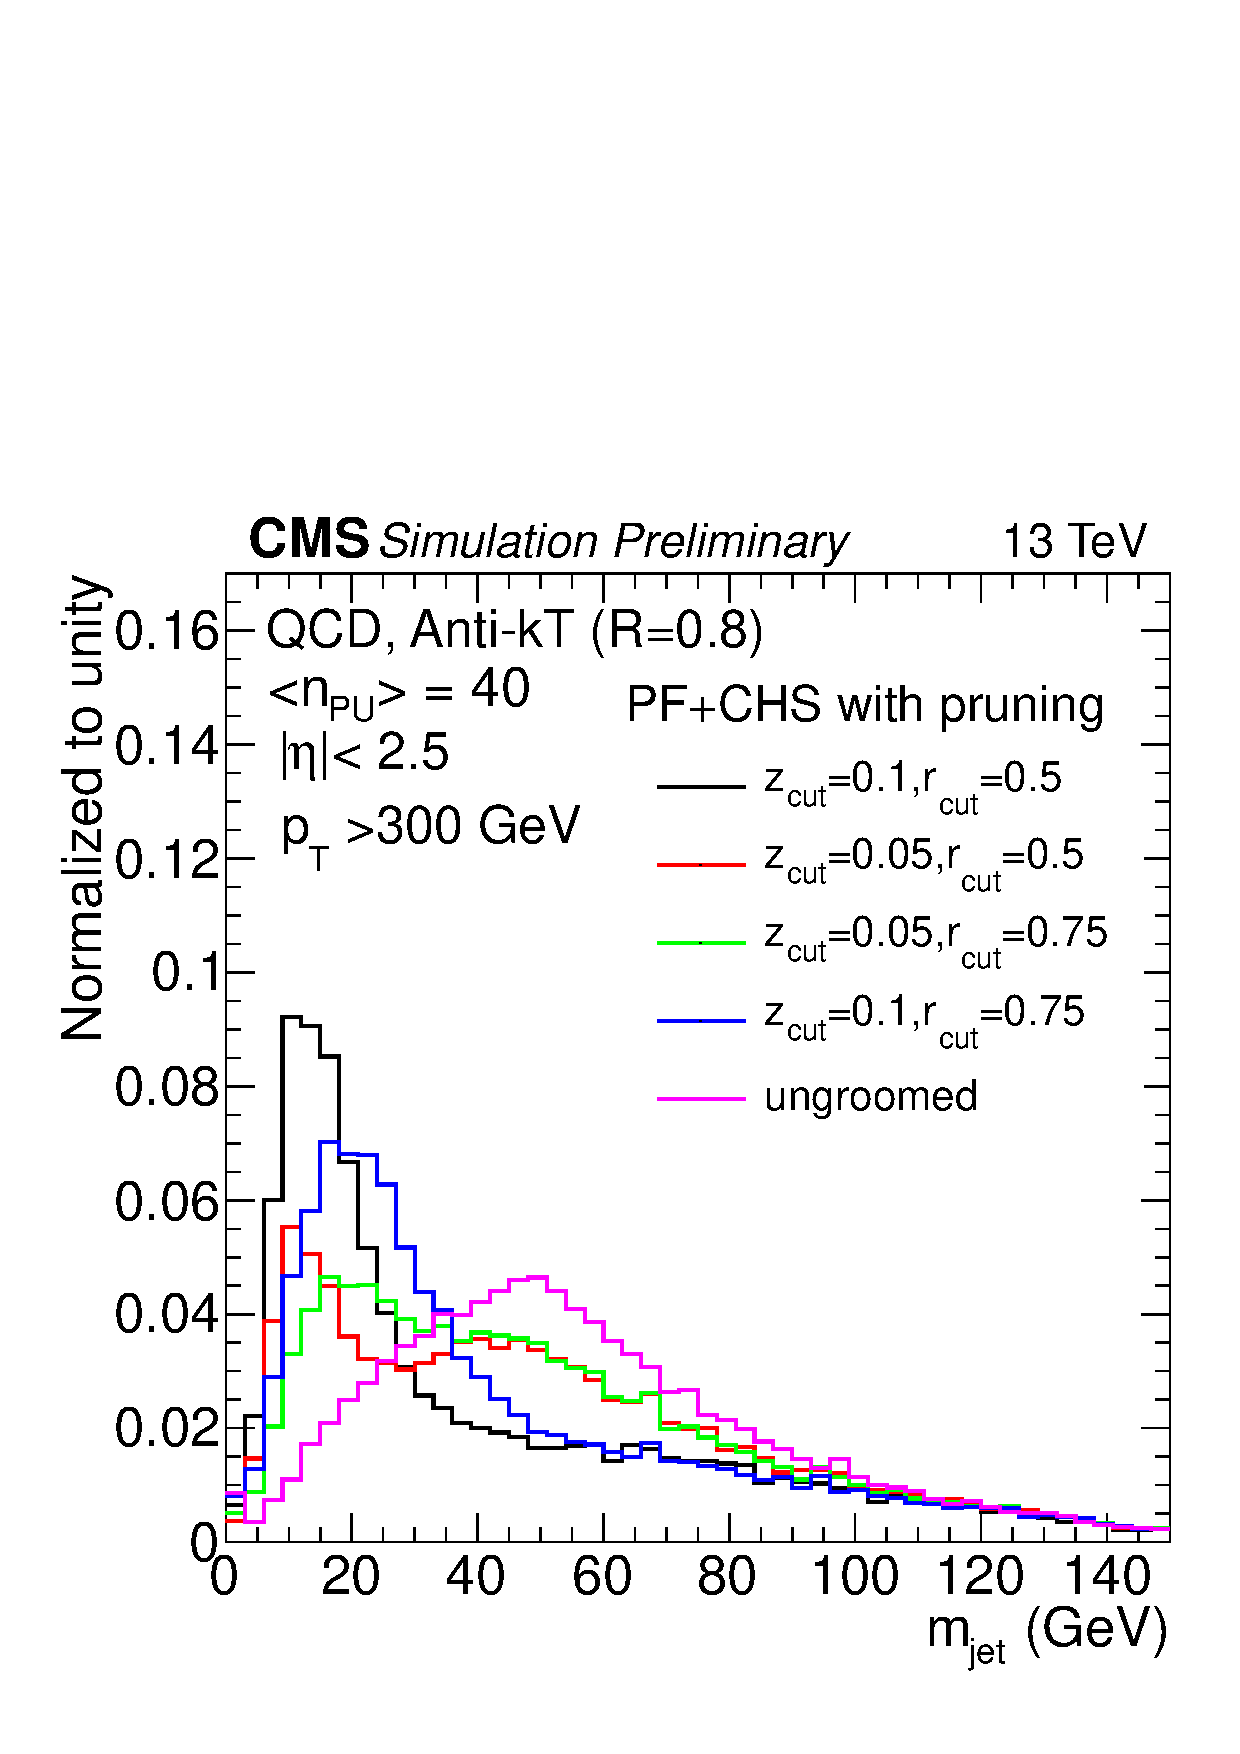
\includegraphics[width=0.6\textwidth]{figures/razor_wtag/1DPFCHS_PR_QCD}
  \caption{Jet mass distribution of QCD jets with $\pt(\textrm{gen}) > 300 \GeV$ for jet pruning
with different parameters, starting from PF jets with charge-hadron subtraction applied. The fully
ungroomed mass distribution is also shown for comparison~\cite{CMS-PAS-JME-14-001}. 
  \label{fig:wtag_jet_pruning}}
\end{figure}

%%%%%%%%%%%%%%%%%%%%%%%%%%%%%%%%%%%%%%%%%%%%%%%%%%%%%%%%%%%%%%%%%%%%%%%%%%%%%%%%%%%%%%%%%%%%%%%%%%%%

\subsection{N-subjettiness}

Requiring the jet mass to be consistent with the $\W$ boson mass already results in a good
discrimination between $\W$- and quark/gluon-initiated jets. We can however still do better. A
boosted QCD jet with a mass around 80\GeV usually originates from a single hard parton and acquires
mass through large angle soft splittings. The energy pattern for this process will differ from the
two-prong pattern that is found in boosted $\W$ jets.  
The set of N-subjettiness observables $\tau_N$~\cite{Thaler:2010tr} aims to exploit this difference
in expected energy flow to differentiate between $\W$- and quark/gluon-initiated jets by counting
the number of hard lobes of energy within a jet.

N-subjettiness is computed under the assumption that the jet has N subjets, and is the
$\pt$-weighted $\Delta R$ distance between each jet constituent and its nearest subjet axis:
\begin{equation}
\tau_N = \frac{1}{R_0 \sum_{k} p_{T, k}} \sum_k p_{T, k} \min (\Delta R_{1,k}, \Delta R_{2,k}, ...
\Delta R_{N,k}),
\end{equation}
where $R_0$ is the original jet distance parameter (0.8 in our case) and $k$ runs over all
constituent particles of the jet. 
The subjet axes are obtained by running the exclusive $k_T$
algorithm~\cite{Ellis:1993tq,Catani:1993hr} using \textsc{FastJet}. 
The exclusive $k_T$ algorithm differs from the inclusive version in two ways: if at a given
clustering step $d_{iB} < \min_j d_{ij}$, then constituent $i$ is discarded, rather than added to
the jet collection; and the clustering stops when the desired number of jets (N) is reached. 
The resulting axes can be further optimized to minimize the N-subjettiness value. In accordance to
the CMS recommendation, we use a “one-pass” optimization of the exclusive $k_T$
axes~\cite{nsubjettiness_fastjet}.

The variables $\tau_N$ quantify the consistency of the jet having N subjets. They have a small
value (close to 0) if the original jet is consistent with having N or fewer subjets, because almost
every jet constituent will be close in $\Delta R$ to its own true subjet. 
As we are interested in discriminating boosted $\W$ bosons, with two subjets, from quark/gluon
jets, which have a single subjet, we will use the variables $\tau_2$ and $\tau_1$, as obtained
from the unpruned CA8 jets. To ensure that the N-subjettiness ratio as computed from the unpruned
jet collection is assigned to the correct pruned jet, we find the highest \pt unpruned jet that is
within $\Delta R = 0.7$ of the considered pruned jet.  
It has been shown that the ratio of the $\tau_N$ variables are better discriminitors than the
separate variables. We will thus require that the ratio $\tau_2 / \tau_1$ is small. The $\tau_2 /
\tau_1$ distribution for highly boosted and longitudinally polarized $\W$ bosons and for inclusive
QCD jets is shown in Fig.~\ref{fig:boost_wtag_tau2tau1}. 

\begin{figure}[htpb]
  \centering
  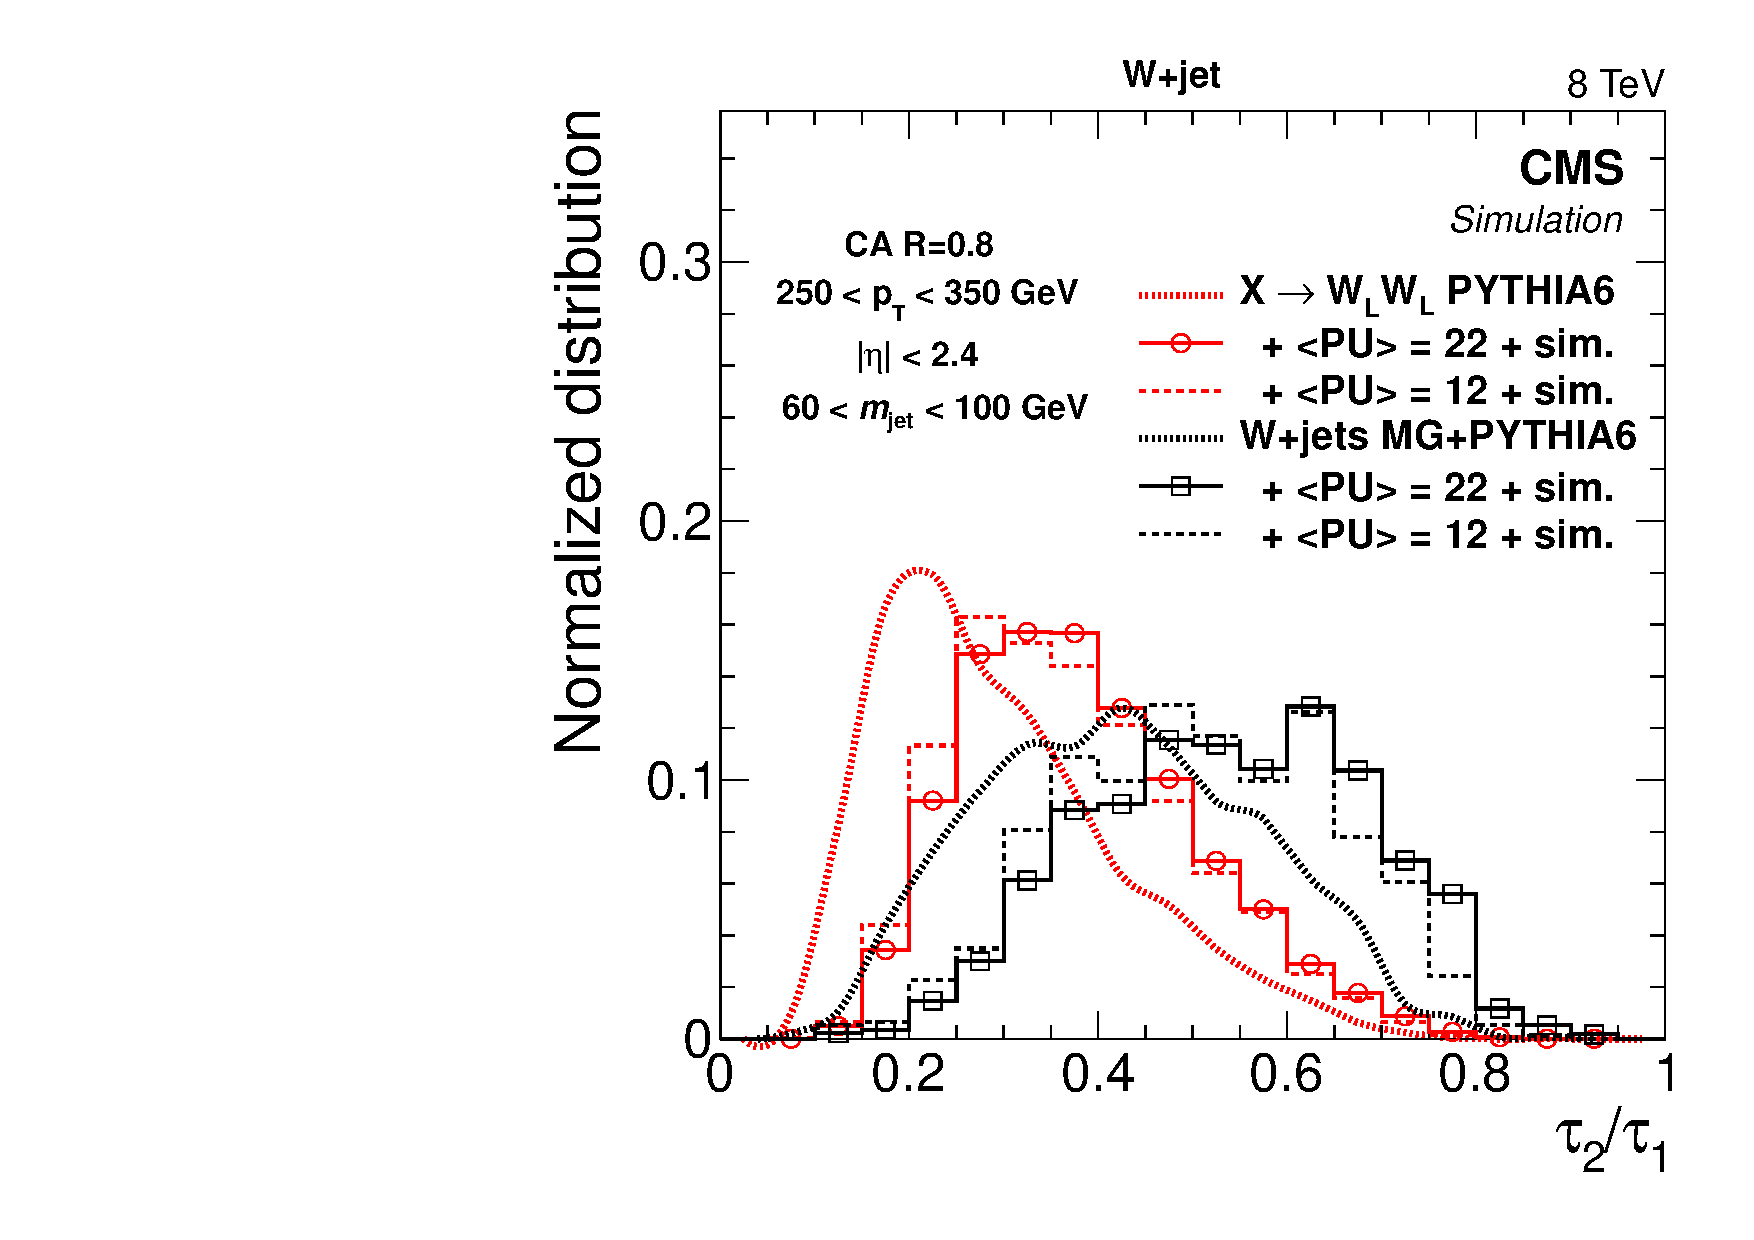
\includegraphics[width=0.7\textwidth]{figures/razor_wtag/tau2tau1_afterMass}
  \caption{Distributions of the N-subjettiness ratio $\tau_2 / \tau_1$ in simulated samples of
highly boosted and longitudinally polarized $\W$ bosons and inclusive QCD jets expected in the
$\W$+jet topology (i.e. with leptonically decaying $\W$ bosons recoiling off a hard jet). 
The distribution is shown after a selection on the pruned jet mass of $60 < m_{\textrm{pruned jet}}
< 100 \GeV$. Note that this is slightly different from what is applied in the razor boost analysis.
Thick dashed lines represent the generator predictions without pileup interactions and without CMS
detector simulation. The histograms are the expected distributions after full CMS simulation with
pileup corresponding to an average number of 12 and 22 interactions~\cite{Khachatryan:2014vla}. 
  \label{fig:boost_wtag_tau2tau1}}
\end{figure}


%%%%%%%%%%%%%%%%%%%%%%%%%%%%%%%%%%%%%%%%%%%%%%%%%%%%%%%%%%%%%%%%%%%%%%%%%%%%%%%%%%%%%%%%%%%%%%%%%%%%

\subsection{\texorpdfstring{$\W$}{W} tagging definitions}

In the razor boost analysis we will emply a boosted $\W$ boson tagger, using the techniques
outlined in the previous sections, to identify events that are consistent with the presence of a
high \pt, hadronically decaying $\W$ boson. 
A given pruned CA8 jet is $\W$ tagged if it has $\pt > 200\GeV$, $|\eta|<2.4$, $70 < m_\textrm{jet}
< 100\GeV$, and the corresponding unpruned jet satisfies $\tau_2 / \tau_1 < 0.5$.
This definition is the same as was used previously in a search for massive resonances in dijet
systems containing jets tagged as W or Z boson~\cite{EXO-12-024,EXO-13-009}. 
The precise definition of this $\W$ tagger is summarized in Table~\ref{tab:Wtag_definition}.

As explained in Section~\ref{sec:boost_strategy}, we will use three control regions to select data
samples enriched in QCD multijet, $t\bar{t}$, and $\W(\rightarrow l \nu)+$jets, in order to help
model the SM backgrounds. QCD multijet and leptonically decaying $\W$+jets events are not expected
to have jets with a two-prong substructure. Therefore, our $\W$ tagging definition will not be very
efficient in selecting these processes. To remedy this, we slightly modify our $\W$ tagger. 
We define $\W$ \textit{anti-tagged} jets by taking the complement of the $\tau_2 / \tau_1$
requirement, and define $\W$ \textit{mass-tagged} jets by dropping that requirement all together. 
These definitions will allow to more efficiently select background processes, while remaining in a
similar kinematic regime. How these taggers will be used exactly will be explained in
Section~\ref{sec:boost_control_selection}. A summary of their definition can be found in
Table~\ref{tab:Wtag_definition} as well. 

\begin{table}[htdp]
\caption{Boosted $\W$ tagging definitions. The input jet collection is either the pruned or unpruned
CA8 jet collection with charge-hadron subtraction applied. }
\vspace{1ex}
\centering
\begin{tabular}{l c c c}
\toprule
& $\W$ tagging & $\W$ anti-tagging & $\W$ mass-tagging  \\
\midrule
\multirow{3}{*}{Pruned} & $\pt > 200$  & $\pt > 200$  & $\pt > 200$\\
& $|\eta| < 2.4$ & $|\eta| < 2.4$ & $|\eta| < 2.4$\\
& $70 < m_{\textrm{jet}}< 100$ & $70 < m_{\textrm{jet}}< 100$ & $70 < m_{\textrm{jet}}< 100$\\
\midrule
Unpruned & $\tau_2 / \tau_1 < 0.5$ & $\tau_2 / \tau_1 \geq 0.5$ & -\\
\bottomrule
\end{tabular}
\label{tab:Wtag_definition}
\end{table}

%%%%%%%%%%%%%%%%%%%%%%%%%%%%%%%%%%%%%%%%%%%%%%%%%%%%%%%%%%%%%%%%%%%%%%%%%%%

%Data/MC scale factors for these definitions are also needed. They are not provided centrally, so we
%derived them ourselves. For more details we refer to section~\ref{sec:wtag_scale_factor}. In that
%section we also show how we derive a FullSim/FastSim scale factor and a scale factor for the W-tag
%fake rate. 


\subsection{\texorpdfstring{$\W$}{W} tagging scale factors \label{sec:wtag_scale_factor}}

It has been observed by previous CMS analyses that the $\W$ tagging efficiency is not the same in
data and in simulation. An example of this is shown on Fig.~\ref{fig:boost_wtag_data_sim}. 
To account for these discrepancies, we need to derive data/MC scale factors corresponding to each
of the $\W$ tagging, $\W$ mass-tagging and $\W$ anti-tagging definitions listed in
Table~\ref{tab:Wtag_definition}. These scale factors are not process-independent. They will be
different for processes that include hadronically decaying $\W$ bosons, such as $t\bar{t}$ or the
signal, compared to processes which do not have $\W$ bosons in their final state, such as QCD
multijet. For processes that do not have real hadronically decaying $\W$ bosons, any tagged jet is
necessarily a misidentified, or \textit{fake}, $\W$ boson tag. For those processes we will speak of
the $\W$ boson tagging fake rate scale factors, where the fake rate is defined as the probability to
tag, with one of the used W tagging definitions, a jet not coming from a hadronically decaying $\W$
boson. 
One last consideration concerns the signal simulation. As the signal is simulated with FastSim, we
need an additional scale factor between FastSim and FullSim. 
In the following subsections every scale factor will be listed in more detail, including how it was
derived and how it will be used in the analysis. 

\begin{figure}[htpb]
  \centering
  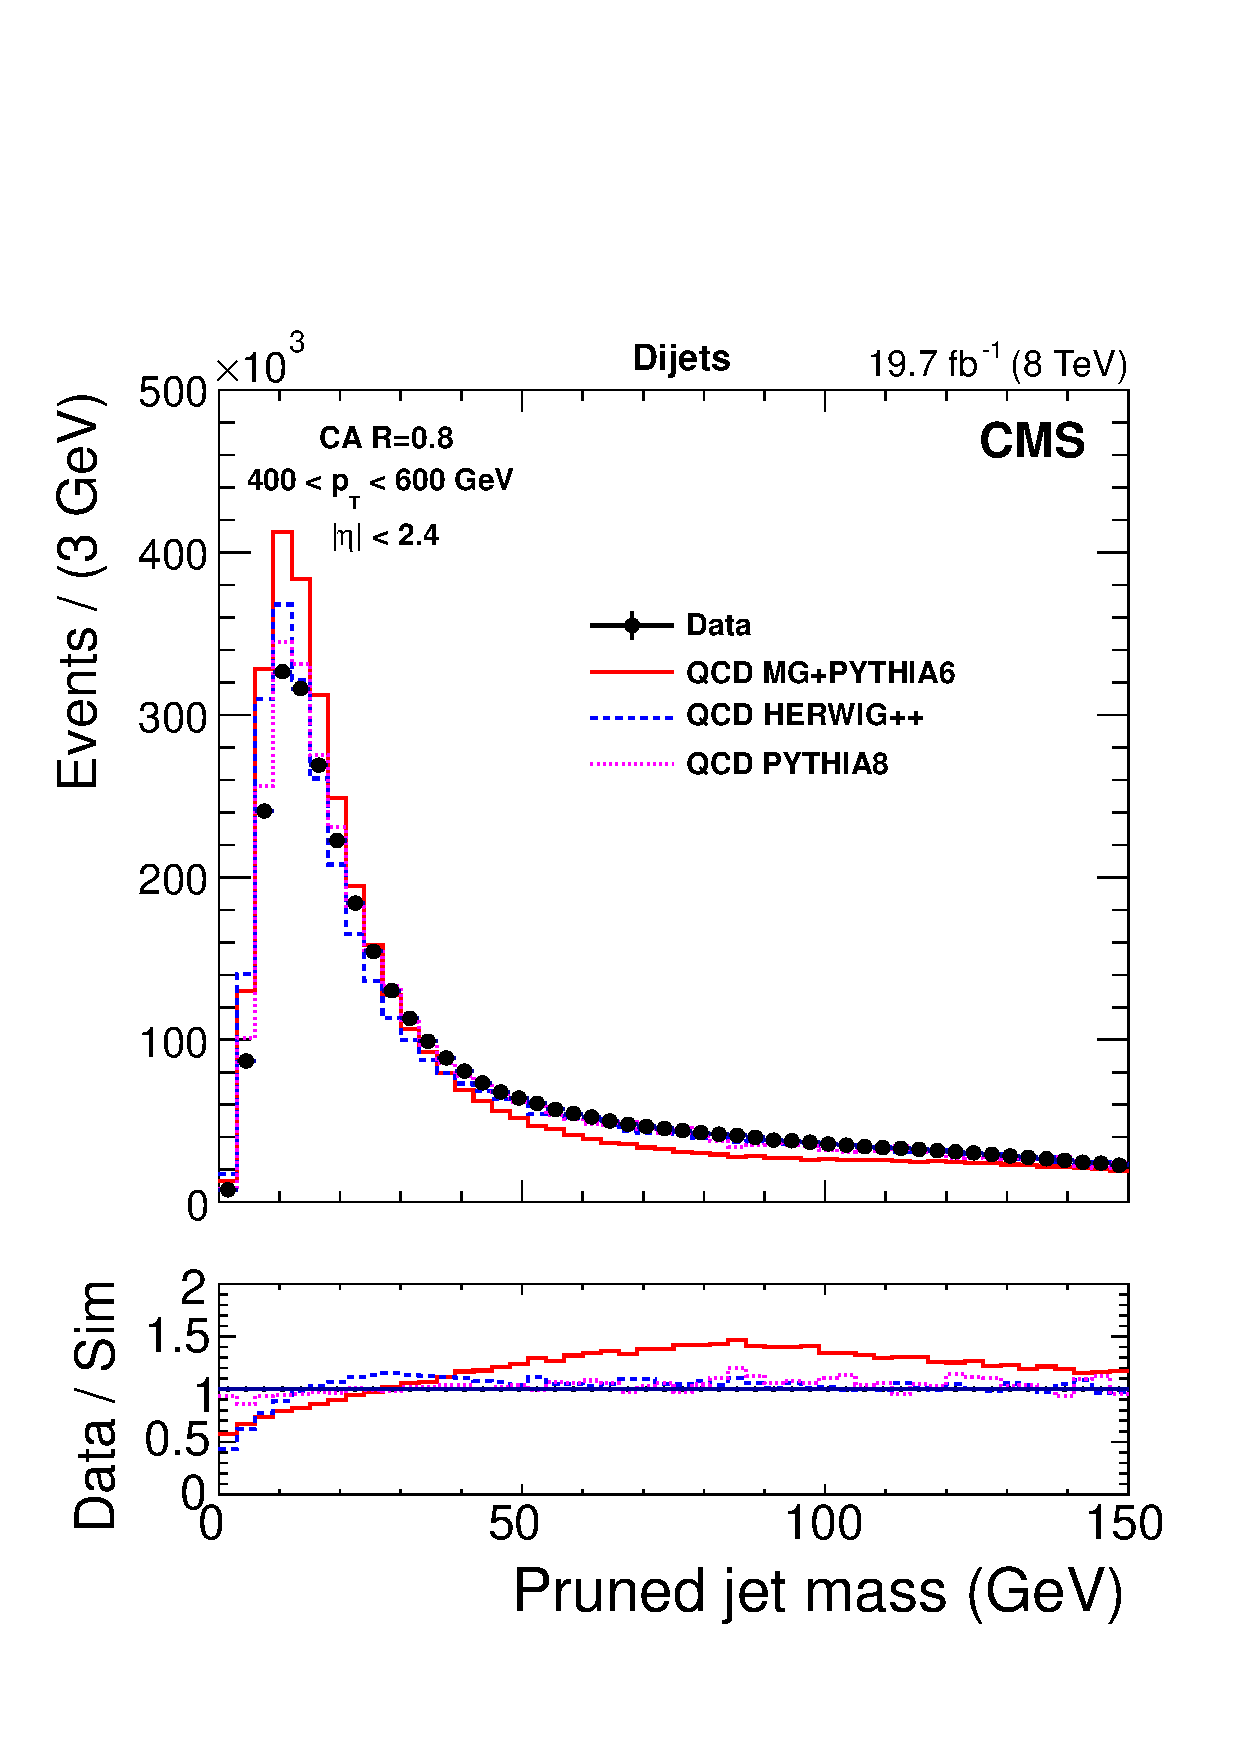
\includegraphics[width=0.48\textwidth]{figures/razor_wtag/substructure_pas_mass_2}
  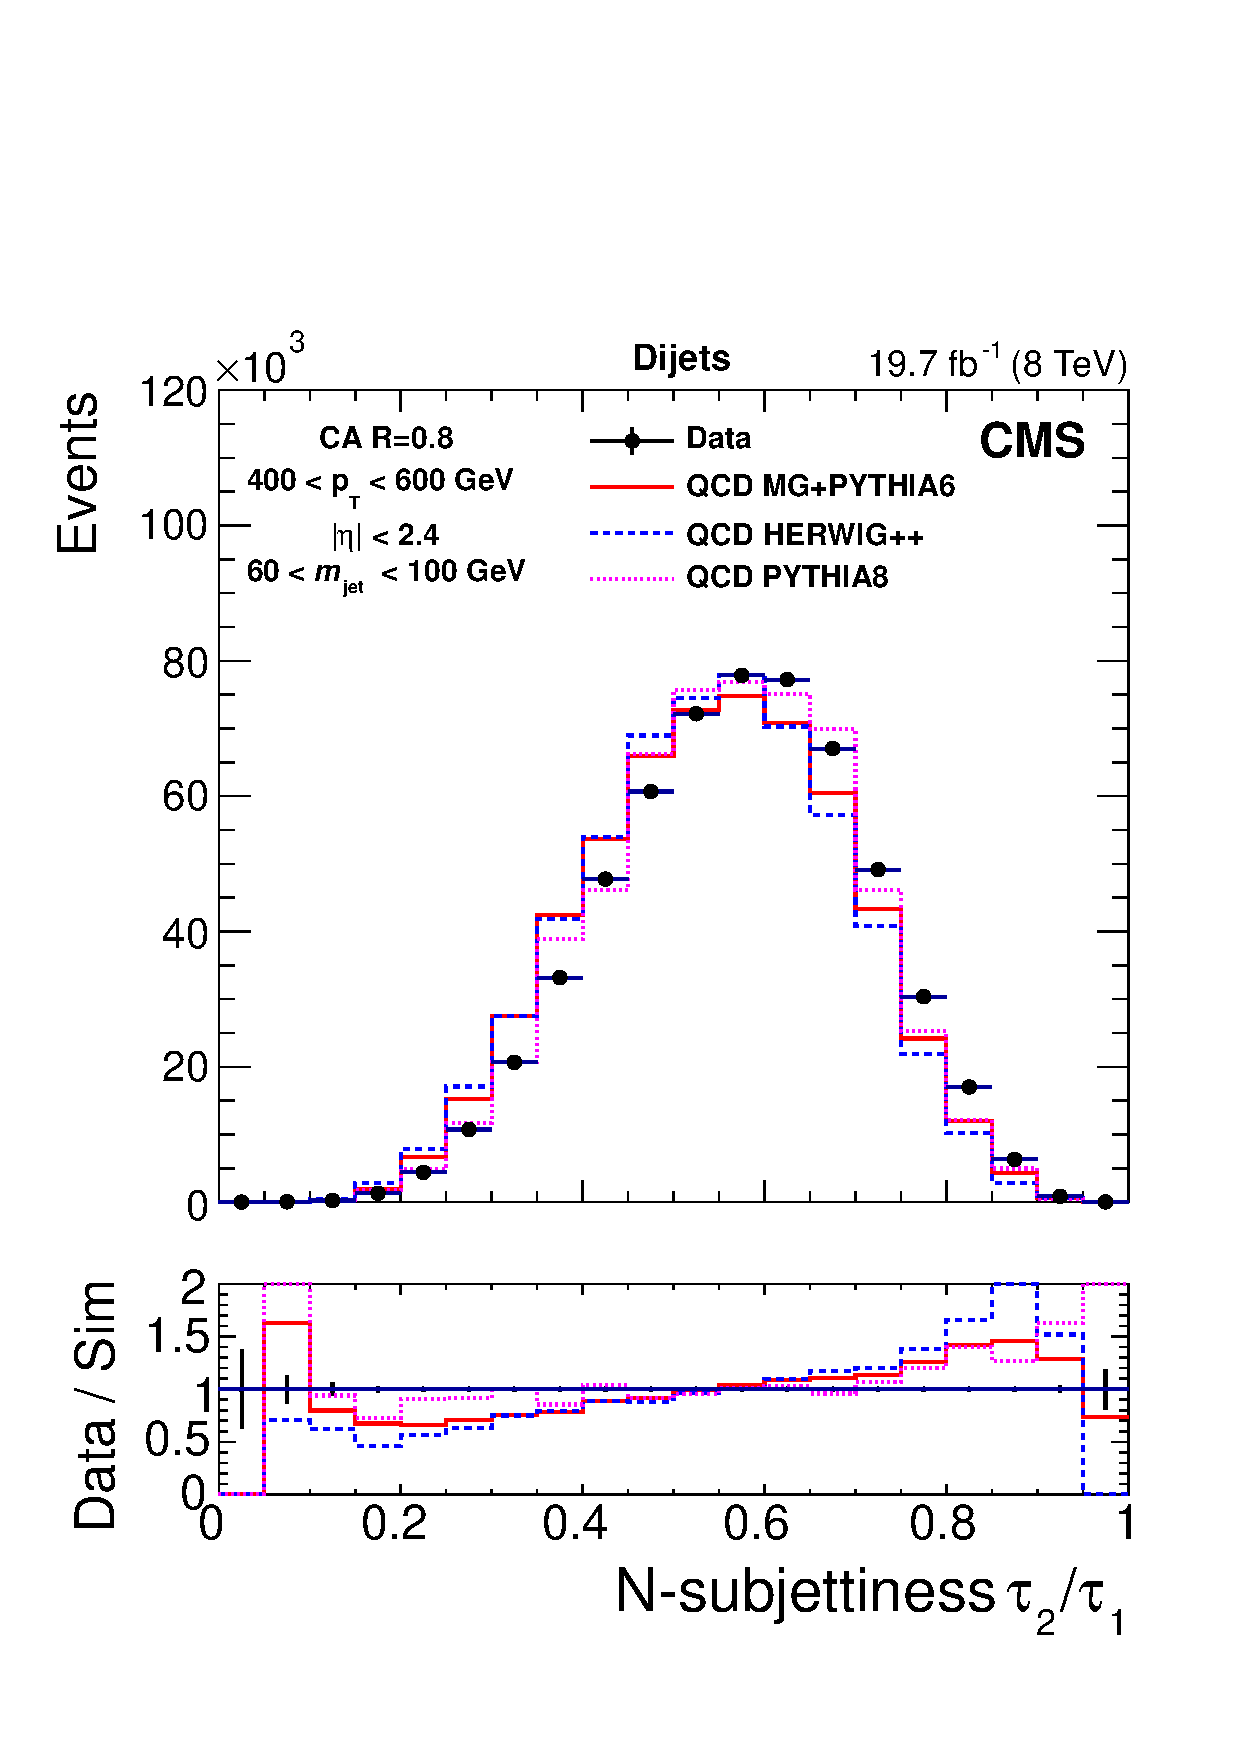
\includegraphics[width=0.48\textwidth]{figures/razor_wtag/substructure_pas_tau21_aftermass_2}
  \caption{
  \label{fig:boost_wtag_data_sim}}  
\end{figure}

\subsubsection{\texorpdfstring{$\W$}{W} boson tag efficiency scale factor \label{sec:wtag_eff_sf}}

The $\W$ boson tag efficiency scale factor will be used to correct processes with real
hadronically decaying $\W$ bosons. For the backgrounds this is mainly for the $t\bar{t}$ process,
but also single top and $t\bar{t}$ in association with a $\W$ or $\cPZ$ boson are considered. This
scale factor is of course also used for the signal processes. 

The $\W$ boson tag efficiency scale factor is only applied to the simulation in the $S$ and $T$
region, see Sections~\ref{sec:boost_signal_selection} and \ref{sec:boost_T_region}, as those are the
selections that utilize the $\W$ tagging definition. It is also only applied to events for which
the $\W$ boson tagged jet is matched (within a cone of $\Delta R = 0.8$) to a generator level
hadronically decaying $\W$ boson. In case no match was found, we apply the $\W$ boson tag fake rate
scale factor. 

As we use the same $\W$ boson tagging definition as was used for the EXO-12-024
paper~\cite{EXO-12-024}, we can directly apply the scale factor that was derived for that study. The
method used to obtain the scale factor is outlined in Ref.~\cite{CMS-PAS-JME-13-006}. 
The $\W$ boson tag efficiency scale factor $SF_{\textrm{Wtag}}$ is given by
\begin{equation}
SF_{\textrm{Wtag}} = 0.86 \pm 0.07 .
\end{equation}

\subsubsection{\texorpdfstring{$\W$}{W} boson tag efficiency FullSim/FastSim scale factor
\label{sec:wtag_eff_fastfull_sf}}

% TODO add the fullsim/fastsim stuff

For our signal samples, which are produced with FastSim, we have derived an additional $\W$ tag
efficiency FullSim/FastSim scale factor, $SF_{\textrm{Full/Fast}}$, which is a function of the \pt
of the CA8 jet. This scale factor corrects for modelling differences in FastSim and FullSim. The
product of $SF_{\textrm{Wtag}}$ and $SF_{\textrm{Full/Fast}}$ will be applied to the signal
simulation. 

To compute the $\W$ boson tag efficiency FullSim/FastSim scale factor we use a sample of $t\bar{t}$
events simulated with FullSim and FastSim. 
We start by determining the $\W$ boson tagging efficiency for both samples using this procedure: 
\begin{enumerate}
\item Filter the events at the generator level, requiring the presence of exactly one hadronically
decaying $\W$ boson. 
\item For the generated $\W$ boson, find the closest CA8 jet, and require that it be within $\Delta
R = 0.8$ from the $\W$ boson. If no such jet exists, the event is discarded.  
\item Require that there be no (generator-level) $\cPqb$ quark from the top quark decay within the
cone of the selected CA8 jet. (We wish to select boosted $\W$ bosons only, not boosted top quarks.)
\item For the events that pass the above selection, consider the $\pt$ distribution of the CA8 jet
at two selection levels:
 \begin{itemize}
   \item no additional selection
   \item $70 < m_\textrm{jet} < 100$\GeV and $\tau_2/\tau_1 < 0.5$
 \end{itemize}
\item By dividing those \pt distributions we obtain the $\W$ boson tagging efficiency. 
\end{enumerate}
To determine the FullSim/FastSim scale factor for the $\W$ boson tagging efficiency, we divide the
efficiencies $\epsilon$ obtained in FullSim and FastSim:
\begin{equation}
SF_{\textrm{Full/Fast}}(\pt) =
\frac{\epsilon_{\textrm{FullSim}}(\pt)}{\epsilon_{\textrm{FastSim}}(\pt)}.
\end{equation}


\subsubsection{\texorpdfstring{$\W$}{W} boson tag fake rate scale factor \label{sec:wtag_fake_sf}}

%To derive the scale factors for the $\W$ boson mass tag fake rate, the $\W$ boson anti-tag fake
%rate, and the $\W$ boson tag fake rate, we use a multijet-enriched control region, defined with the
%following selection:
The $\W$ boson tag fake rate scale factor is meant to correct processes that do not have
hadronically decaying $\W$ bosons in their final state. To derive the scale factor we will thus need
to obtain a sample of events containing misidentified $\W$ boson jets. 
We will use a multijet-enriched control region, defined with the following selection:
\begin{itemize}
\item no leptons
\item no $\cPqb$ tagged jets
\item at least 3 AK5 jets
\item at least one AK5 jet with $\pt>200$\GeV
\item $\Delta\phi_{min} < 0.3$
%TODO define deltaphimin somewhere
\end{itemize}
This selection is similar to the baseline selection employed in the rest of the analysis. The
kinematic regime, and the composition of the sample will thus also be similar. 

To obtain the fake rates $\epsilon$ for $\W$ boson tagging we use the leading CA8 jet in each
event, and check whether it is tagged by the $\W$ boson tagger. After obtaining the
fake rates in both data and simulation, we compute the scale factor as,
\begin{equation}
SF_\textrm{Wtag,fake}(\pt) =
\frac{\epsilon^{\textrm{data}}(\pt)}{\epsilon^{\textrm{simulation}}(\pt)}.
\end{equation}  

In the calculation of the uncertainties on this scale factor we include the statistical uncertainty,
as well as the trigger efficiency and jet energy scale uncertainties. 

This SF is applied in the $S$ and $T$ region,
to all simulated samples without real hadronically decaying W bosons (e.g. multijet,
$W\rightarrow\ell\nu$+jets, ...).

\subsubsection{\texorpdfstring{$\W$}{W} boson mass-tag fake rate scale factor
\label{sec:wmasstag_fake_sf}}
This SF corresponds to the $\W$ tag
definition as used in the $W$ region, i.e. mass-tagging, and is thus only applied to the simulated
samples in the $W$ region. 
The $W$ region is dominated by leptonically decaying $\W$ bosons. The mass-tagged jet, therefore,
originates from a q/g jet, which is the reason for deriving this SF in a multijet-enriched
region. 
\subsubsection{\texorpdfstring{$\W$}{W} boson anti-tag fake rate scale factor
\label{sec:wantitag_fake_sf}}

This SF corresponds to the $\W$ tag
definition as used in the $Q$ region, i.e. anti-tagging. It is applied to the simulated samples in
the $Q$ region.

% TODO explain the wiggle

%%%%%%%%%%%%%%%%%%%%%%%%%%%%%%%%%%%%%%%%%%%%%%%%%%%%%%%%%%%%%%%%%%%%%%%%%%%%%%%%%%%%%%%%%%%%%%%%%%%%


% 
% \subsection[W tag scale factors]{$\PW$ tag scale factors \label{sec:Wtag_SF}}
% 
% It has been observed by several analyses that the $\PW$ tagging efficiency is not the same in data
% and simulation. 
% In order to account for this, a scale factor with corresponding uncertainty is applied to the
% simulated events. 
% As we use the official $\PW$ tagger, we can immediately use the already approved scale factor of
% $0.86 \pm 0.07$~\cite{EXO-12-024}. 
% 
% Details on the derivation of data/simulation scale factors for the $\PW$ mass-tag and $\PW$ anti-tag
% fake rate, as well as on the fake rate and FullSim/FastSim SF associated with the full $\PW$ tagger,
% are giving in the next subsections. 

% \subsubsection{Scale factors for only mass-tagged and anti-tagged $\PW$s}
% 
% We use mass-tagged $\PW$s ($Y$s) and anti-tagged $\PW$s while defining our $W$ and $Q$ control
% regions.  
% These regions are dominated by processes that do not have real hadronically decaying $\PW$ bosons.
% All CA8 jets that pass the $Y$ or $aW$ selection imposed in these regions, are thus in fact
% $\cPq/\cPg$-jets that are misidentified, or \textit{fake}. Therefore, we will use a multijet
% enriched control region to derive scale factors and uncertainties corresponding to the $Y$ and $aW$
% tagger definitions.
% 
% The control region is defined with the following selection:
% \begin{itemize}
% \item 0 loose leptons
% \item 0 CSVL btagged jets
% \item $\geq 3$ AK5 jets
% \item $p_T($jet1$)>200$GeV
% \item no $M_R$, $R^2$ cuts
% \item $\Delta\phi_{min} < 0.3$
% \end{itemize}
% This selection is purpusefully as close as possible to the selection we make in our analysis.
% We obtain the mass-tagged $\PW$ and anti-tagged $\PW$ fake rate using the leading CA8 jet in each
% event.  
% After obtaining the probability of $\PW$ mass-tagging or anti-tagging the $\cPq/\cPg$ jets in this
% control region for both data and MC, we obtain the scale factor from the ratio of data to MC fake
% rates.  Figure~\ref{fig:YaWeff} shows the $\PW$ mass- and anti-tagging fake rate in data and
% simulation. Figure~\ref{fig:YaWSF} shows the scale factors versus CA8 jet \pt for mass-tagged and
% anti-tagged $\PW$s.
% 
% \begin{figure}[htbp]
% \centering
% \includegraphics[width=0.49\textwidth]{figures/SF_Wtag_anti/Wtag_eff_ratio_pt_Wmass_all_Data}
% \includegraphics[width=0.49\textwidth]{figures/SF_Wtag_anti/Wtag_eff_ratio_pt_Wmass_all_MC}
% 
% \includegraphics[width=0.49\textwidth]{figures/SF_Wtag_anti/Wtag_eff_ratio_pt_antitagged_all_Data}
% \includegraphics[width=0.49\textwidth]{figures/SF_Wtag_anti/Wtag_eff_ratio_pt_antitagged_all_MC}
% \caption{Misidentification probability for only mass-tagged $\PW$s (top) and anti-tagged $\PW$s
% (bottom) versus CA8 jet \pt obtained from a QCD control region as described in the text. On the left
% we show the fake rate in data, while on the right we show the fake rate in simulation. Uncertainties
% are statistical only.
% \label{fig:YaWeff}}
% \end{figure}
% 
% \begin{figure}[htbp]
% \centering
% \includegraphics[width=0.49\textwidth]{figures/SF_Wtag_anti/Wtag_SF_SF_Wmass_pt}
% \includegraphics[width=0.49\textwidth]{figures/SF_Wtag_anti/Wtag_SF_SF_antitagged_pt}
% \caption{Scale factors for the fake rate for mass-tagged $\PW$s (left) and anti-tagged $\PW$s
% (right) versus CA8 jet \pt obtained from a QCD control region as described in the text.
% Uncertainties are statistical only.
% \label{fig:YaWSF}}
% \end{figure}
% 
% As we can see from these figures, there is a drop in the scale factor around a \pt of 300\GeV. 
% This is a result of a residual mismodeling of the trigger efficiency, as is explained in more detail
% in appendix~\ref{app:wiggle}. 
% Given that we understand the origin of this wiggle, we decide to keep the binning quite fine in that
% region, so that we can correct for the effect. 
% The scale factors with the final binning are shown in figure~\ref{fig:YaWSF_syst}, and are also
% listed in tables~\ref{tab:SF_Wmass} and \ref{tab:SF_Wantitagging} with the breakdown of the
% statistical and systematic uncertainties. The included systematic uncertainties are the jet energy
% scale uncertainties for both AK5 and CA8 jets, and the trigger efficiency uncertainties. All three
% uncertainties are varied up (down) at the same time to get the overall up (down) systematic
% uncertainty.
% A summary of the two scale factors, mass-tagged and anti-tagged, with their total uncertainty is
% shown in table~\ref{tab:SF_Wantitagging_summary}.  
% 
% \begin{figure}[htbp]
% \centering
% \includegraphics[width=0.49\textwidth]{figures/SF_Wtag_anti/SF_Wmass}
% \includegraphics[width=0.49\textwidth]{figures/SF_Wtag_anti/SF_antitagging}
% \caption{Scale factors for the fake rate of mass-tagged $\PW$s (left) and anti-tagged $\PW$s (right)
% versus CA8 jet \pt obtained from a QCD control region as described in the text. The error bars
% depict the statistical uncertainties, while the error band shows the total uncertainty. 
% \label{fig:YaWSF_syst}}
% \end{figure}
% 
% \begin{table}[htbp]
% \centering
% \caption{Scale factors for fake rate of having a q/g initiated CA8 jet with mass within the W mass
% window \label{tab:SF_Wmass}}
% \vspace{1ex}
% \begin{tabular}{|c|c|c|c|c|}
% \hline
% CA8 jet \pt & $SF_{Wmasstag}$ & stat uncertainty & syst uncertainty & total uncertainty \\
% \hline
% $[200 - 220]$ & 1.144 & 0.050 & 0.012  & 0.052\\
% $[220 - 240]$ & 1.118 & 0.028 & 0.024  & 0.037\\
% $[240 - 260]$ & 1.193 & 0.024 & 0.008  & 0.025\\
% $[260 - 280]$ & 1.250 & 0.018 & 0.015  & 0.023\\
% $[280 - 300]$ & 1.273 & 0.017 & 0.021  & 0.027\\
% $[300 - 320]$ & 1.126 & 0.013 & 0.010  & 0.017\\
% $[320 - 340]$ & 1.199 & 0.012 & 0.017  & 0.021\\
% $[340 - 360]$ & 1.298 & 0.013 & 0.007  & 0.015\\
% $[360 - 380]$ & 1.327 & 0.016 & 0.008  & 0.017\\
% $[380 - 400]$ & 1.339 & 0.025 & 0.007  & 0.026\\
% $[400 - 500]$ & 1.339 & 0.012 & 0.005  & 0.013\\
% $[500 - ]$    & 1.370 & 0.011 & 0.001  & 0.011\\
% \hline
% \end{tabular}
% \end{table}
% 
% \begin{table}[htbp]
% \centering
% \caption{Scale factors for $\PW$ anti-tag fake rate \label{tab:SF_Wantitagging}}
% \vspace{1ex}
% \begin{tabular}{|c|c|c|c|c|}
% \hline
% CA8 jet \pt & $SF_{Wantitag}$ & stat uncertainty & syst uncertainty & total uncertainty \\
% \hline
% $[200 - 220]$ & 1.217 & 0.072 & 0.032  & 0.078\\
% $[220 - 240]$ & 1.186 & 0.037 & 0.046  & 0.059\\
% $[240 - 260]$ & 1.216 & 0.033 & 0.011  & 0.034\\
% $[260 - 280]$ & 1.319 & 0.024 & 0.019  & 0.031\\
% $[280 - 300]$ & 1.479 & 0.022 & 0.037  & 0.043\\
% $[300 - 320]$ & 1.203 & 0.017 & 0.015  & 0.023\\
% $[320 - 340]$ & 1.244 & 0.016 & 0.026  & 0.030\\
% $[340 - 360]$ & 1.409 & 0.019 & 0.015  & 0.024\\
% $[360 - 380]$ & 1.448 & 0.022 & 0.020  & 0.030\\
% $[380 - 400]$ & 1.472 & 0.033 & 0.014  & 0.035\\
% $[400 - 500]$ & 1.487 & 0.017 & 0.012  & 0.021\\
% $[500 - ]$    & 1.505 & 0.014 & 0.004  & 0.015\\
% \hline
% \end{tabular}
% \end{table}
% 
% \begin{table}[htbp]
% \centering
% \caption{Summary of scale factors for efficiency to have a CA8 jet with mass within the W-window;
% and for W anti-tag fake rate \label{tab:SF_Wantitagging_summary}}
% \vspace{1ex}
% \begin{tabular}{|c|c|c|}
% \hline
% CA8 jet \pt & $SF_{Wmasstag}$ & $SF_{Wantitag}$ \\
% \hline
% $[200 - 220]$ & $1.14 \pm 0.06$ & $1.22 \pm 0.08$ \\
% $[220 - 240]$ & $1.12 \pm 0.04$ & $1.19 \pm 0.06$ \\
% $[240 - 260]$ & $1.19 \pm 0.03$ & $1.22 \pm 0.04$ \\
% $[260 - 280]$ & $1.25 \pm 0.03$ & $1.32 \pm 0.04$ \\
% $[280 - 300]$ & $1.27 \pm 0.03$ & $1.38 \pm 0.05$ \\
% $[300 - 320]$ & $1.13 \pm 0.02$ & $1.20 \pm 0.03$ \\
% $[320 - 340]$ & $1.20 \pm 0.03$ & $1.24 \pm 0.03$ \\
% $[340 - 360]$ & $1.30 \pm 0.02$ & $1.41 \pm 0.03$ \\
% $[360 - 380]$ & $1.33 \pm 0.02$ & $1.45 \pm 0.03$ \\
% $[380 - 400]$ & $1.34 \pm 0.03$ & $1.47 \pm 0.04$ \\
% $[400 - 500]$ & $1.34 \pm 0.02$ & $1.49 \pm 0.03$ \\
% $[500 - ]$    & $1.37 \pm 0.02$ & $1.51 \pm 0.02$ \\
% \hline
% \end{tabular}
% \end{table}
% 
% 
% \subsubsection{Scale factor for $\PW$ boson tag fake rate}
% 
% As explained before, we are using the $\PW$-tagger as used in EXO-12-024, which comes with a
% data/simulation scale factor. 
% This scale factor should only be applied to processes which have an actual $\PW$, such as signal
% samples and $t\bar{t}+$jets. 
% CA8 jets that pass the $\PW$-tag requirements in QCD multijet or leptonically decaying $\PW$+jets
% events are `fake' or misidentified $\PW$'s. 
% For these we cannot apply the $\PW$-tag efficiency scale factor, but should apply a scale factor for
% the $\PW$ tag fake rate. 
% In JME-13-006, a measurement of the $\PW$ fake rate is done, and a Data/MC comparison is shown. 
% As the fake rate depends on the composition of the selected event sample, it is recommended,
% however, to derive the scale factor analysis by analysis, rather than having one single scale
% factor. 
% This is what we have done as well. 
% 
% We used the same control region as in the previous section, which is close to our signal region. The
% $M_R$ and $R^2$ cuts are again not applied in order to increase the statistical power of the control
% sample. 
% The procedure is also the same as explained in the previous section. We determine the probability to
% tag the highest \pt CA8 jet as a $\PW$ (using the standard $\PW$-tagger as defined in
% table~\ref{tab:Wtag_EXO}), in both data and simulation, and derive the scale factor from the ratio
% of both. 
% 
% In figure~\ref{fig:W_fake_eff} we show the probability to tag a CA8 jet as a $\PW$, i.e. the fake
% rate, in the multijet control region, for both data and simulation. 
% The resulting scale factor is shown in figure~\ref{fig:W_fake_SF} and table~\ref{tab:W_fake_SF}. The
% considered uncertainties are the statistical precision, and the jet energy scale and trigger
% efficiency uncertainties. 
% 
% \begin{figure}[htbp]
% \centering
% \includegraphics[width=0.49\textwidth]{figures/SF_Wfake/Wtag_eff_ratio_pt_tagged_all_Data}
% \includegraphics[width=0.49\textwidth]{figures/SF_Wfake/Wtag_eff_ratio_pt_tagged_all_MC}
% \caption{Efficiency for tagged $W$s versus CA8 jet \pt in Data (left) and MC (right) for the
% multijet control region listed in the text.
% \label{fig:W_fake_eff}}
% \end{figure}
% 
% \begin{figure}[htbp]
% \centering
% \includegraphics[width=0.49\textwidth]{figures/SF_Wfake/SF_Wfake}
% \caption{Scale factor for $\PW$ fake rate, derived by comparing the efficiency to tag a CA8 jet
% versus \pt for both data and simulation in a QCD control region as described in the text. The error
% bars depict the statistical uncertainties, while the error band shows the total uncertainty. 
% \label{fig:W_fake_SF}}
% \end{figure}
% 
% \begin{table}[htbp]
% \centering
% \caption{Summary of scale factors for $\PW$-tag efficiency fake rate. Uncertainties include the
% statistical and systematic uncertainty. \label{tab:W_fake_SF}}
% \vspace{1ex}
% \begin{tabular}{|c|c|}
% \hline
% CA8 jet \pt & $SF_{\textrm{Wfake}}$ \\
% \hline
% $[200 - 220]$ & $1.04 \pm 0.07$ \\
% $[220 - 240]$ & $1.01 \pm 0.04$ \\
% $[240 - 260]$ & $1.16 \pm 0.04$ \\
% $[260 - 280]$ & $1.16 \pm 0.03$ \\
% $[280 - 300]$ & $1.15 \pm 0.03$ \\
% $[300 - 320]$ & $1.03 \pm 0.02$ \\
% $[320 - 340]$ & $1.14 \pm 0.02$ \\
% $[340 - 360]$ & $1.17 \pm 0.02$ \\
% $[360 - 380]$ & $1.18 \pm 0.03$ \\
% $[380 - 400]$ & $1.18 \pm 0.03$ \\
% $[400 - 500]$ & $1.15 \pm 0.02$ \\
% $[500 - ]$    & $1.18 \pm 0.02$ \\
% \hline
% \end{tabular}
% \end{table}
% 
% 
% \subsubsection{FullSim/FastSim scale factor for $\PW$-tagging efficiency}
% 
% The Data/MC scale factor to correct for the difference in $\PW$ tagging efficiency is derived using
% FullSim, and is thus only valid for FullSim samples. 
% As our signal scans are made with FastSim, we need to derive an additional FullSim/FastSim scale
% factor to account for the different modeling of jets, jet substructure, et cetera. 
% To study the differences and derive the scale factor, we use a $t\bar{t}$ sample, which has been
% processed with both FullSim and FastSim.
% A comparison of the pruned jet mass, and N-subjettiness variables $\tau_1$, $\tau_2$ and
% $\tau_2/\tau_1$ (both before and after cutting on the pruned jet mass), are shown in
% figures~\ref{fig:FastFull_jmass}-\ref{fig:FastFull_tau21}. 
% 
% \begin{figure}
% \centering
% 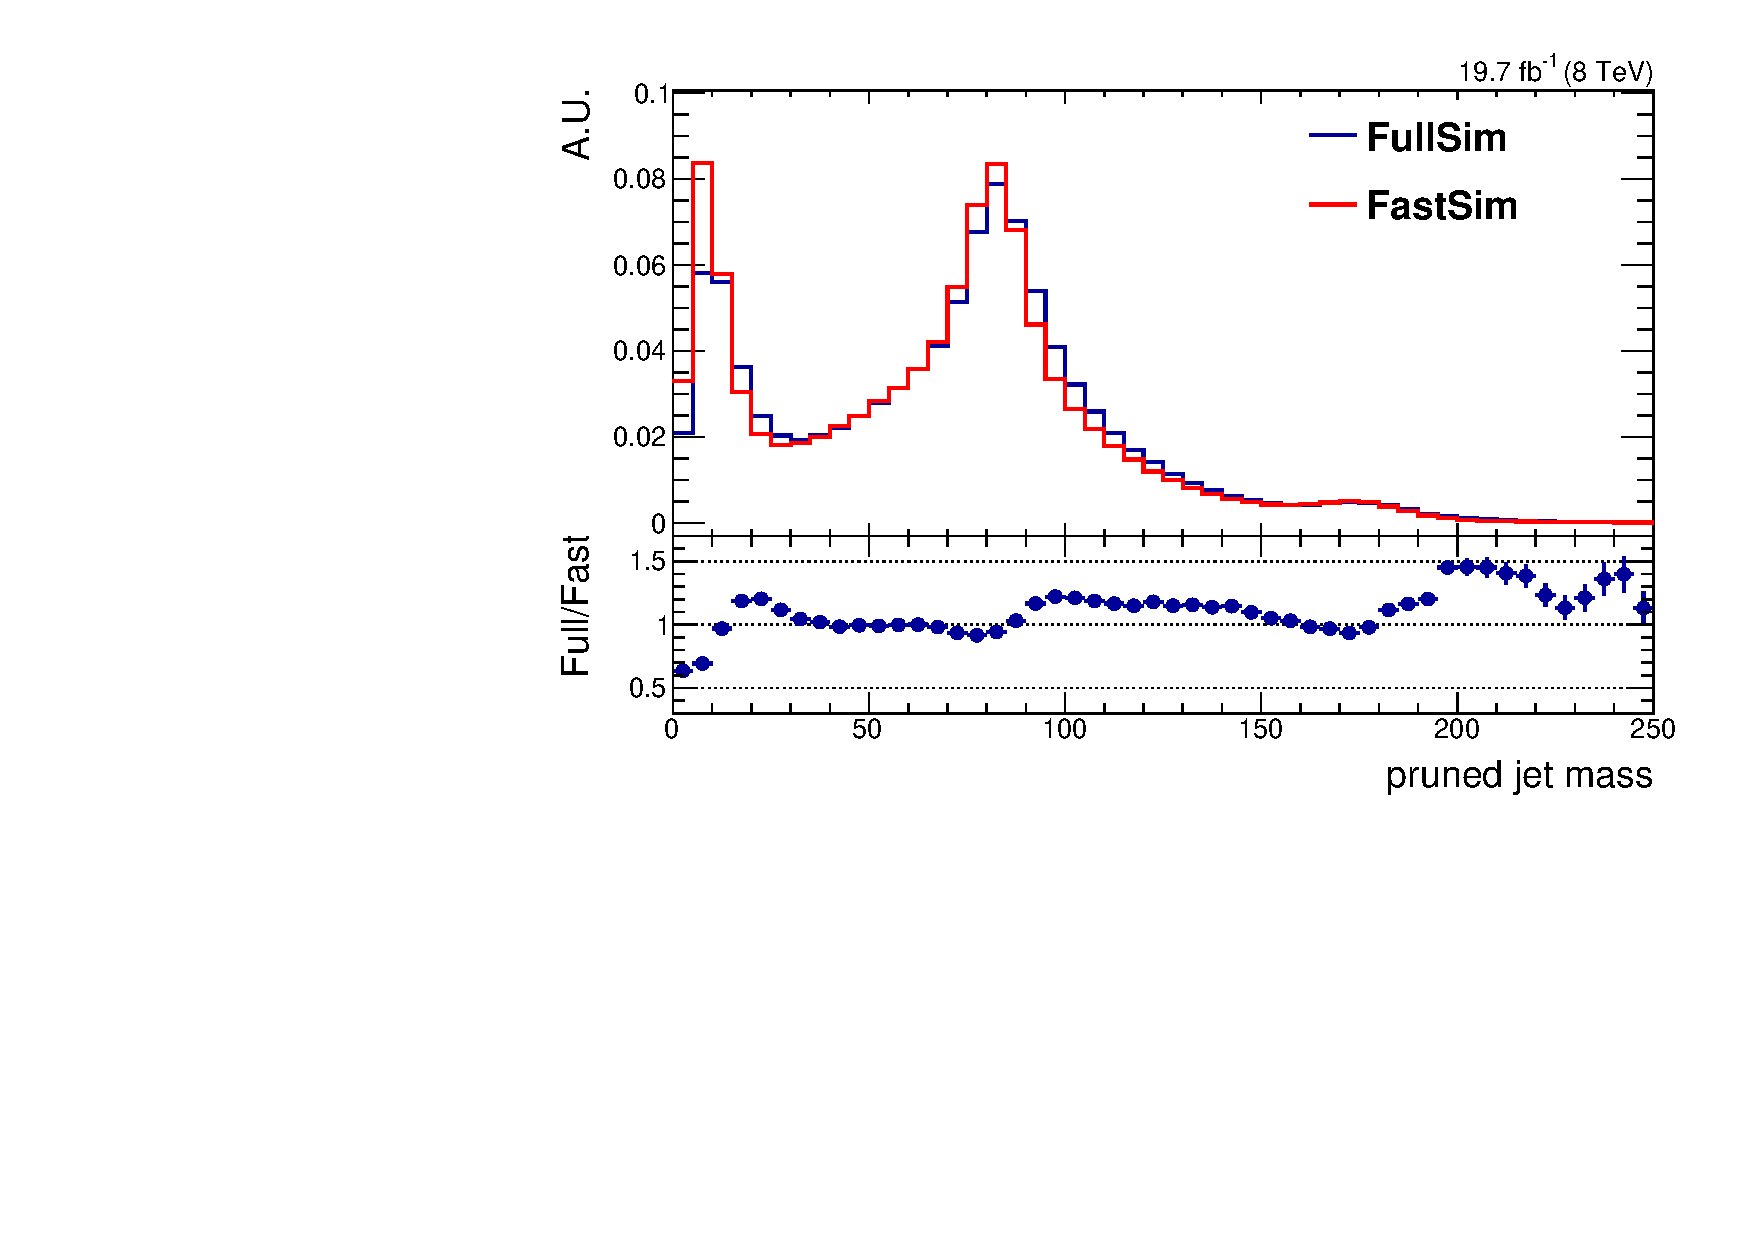
\includegraphics[width=0.7\textwidth]{figures/SF_Wtag_FullFast/FastFull_comparison_TTJets_jmass}
% \caption{Pruned jet mass distribution for FastSim and FullSim $t\bar{t}$. 
% \label{fig:FastFull_jmass}}
% \end{figure}
% 
% \begin{figure}[p]
% 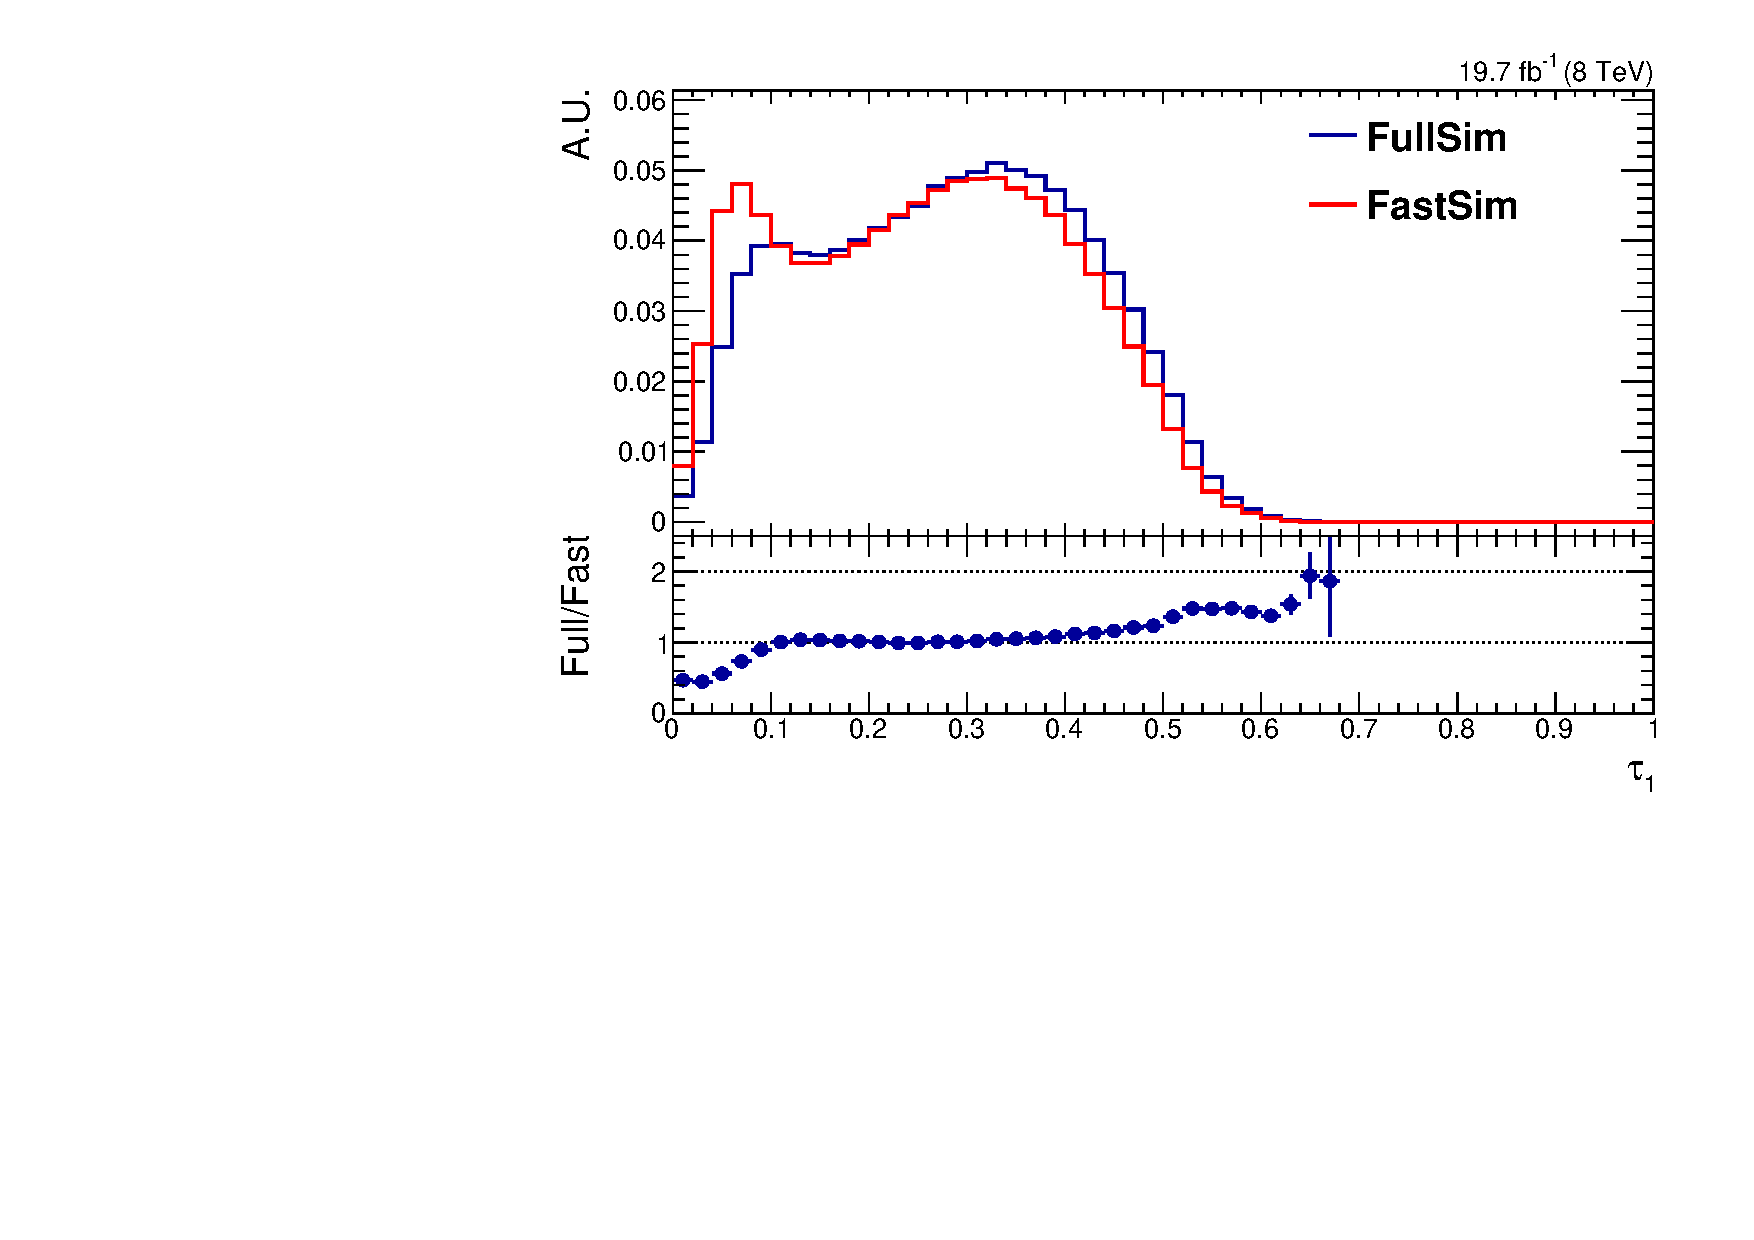
\includegraphics[width=0.49\textwidth]{figures/SF_Wtag_FullFast/FastFull_comparison_TTJets_tau1}
% 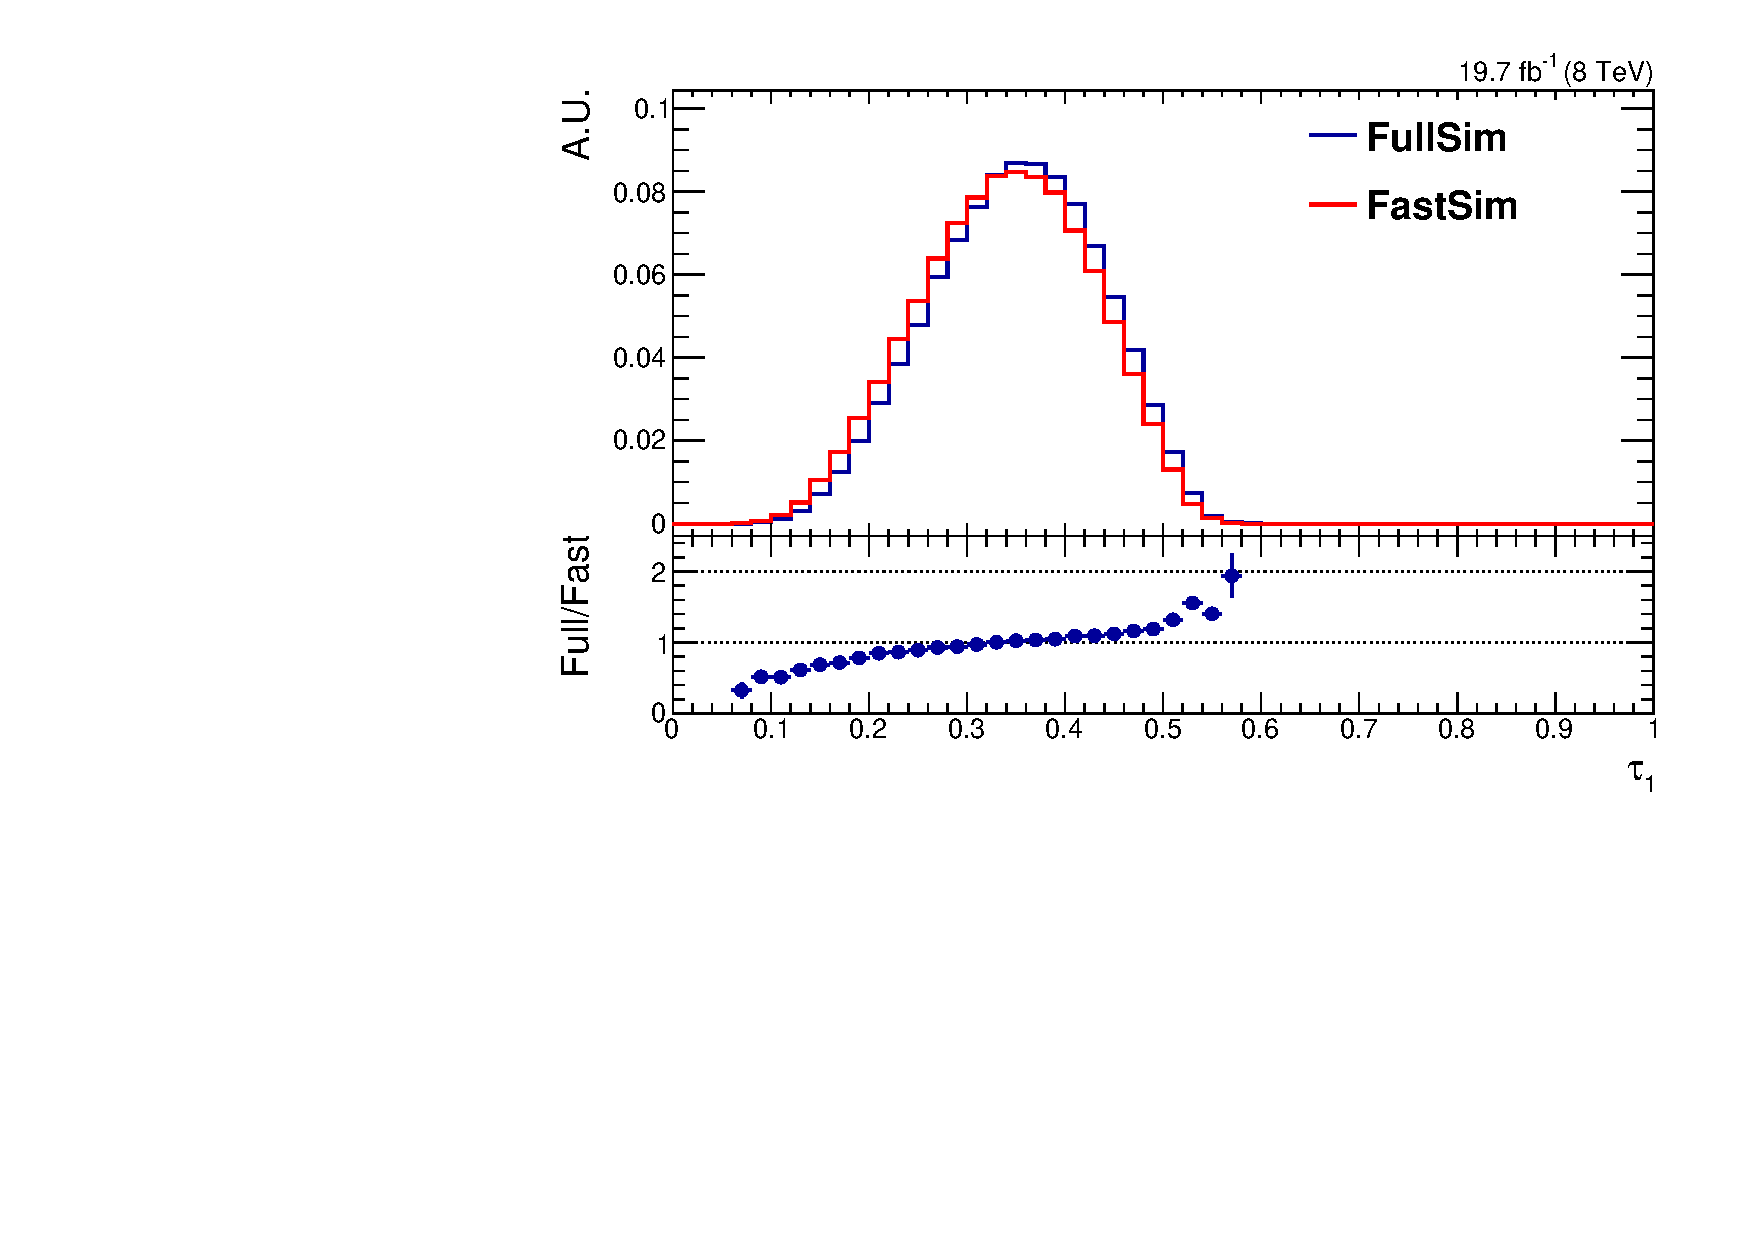
\includegraphics[width=0.49\textwidth]{
% figures/SF_Wtag_FullFast/FastFull_comparison_TTJets_tau1_masscut}
% \caption{Distribution of $\tau_1$ before (left) and after (right) requiring $70 <
% m_{\textrm{jet}}^{\textrm{pruned}} < 100$\GeV, for FastSim and FullSim $t\bar{t}$.
% \label{fig:FastFull_tau1}}
% \end{figure}
% 
% \begin{figure}[p]
% 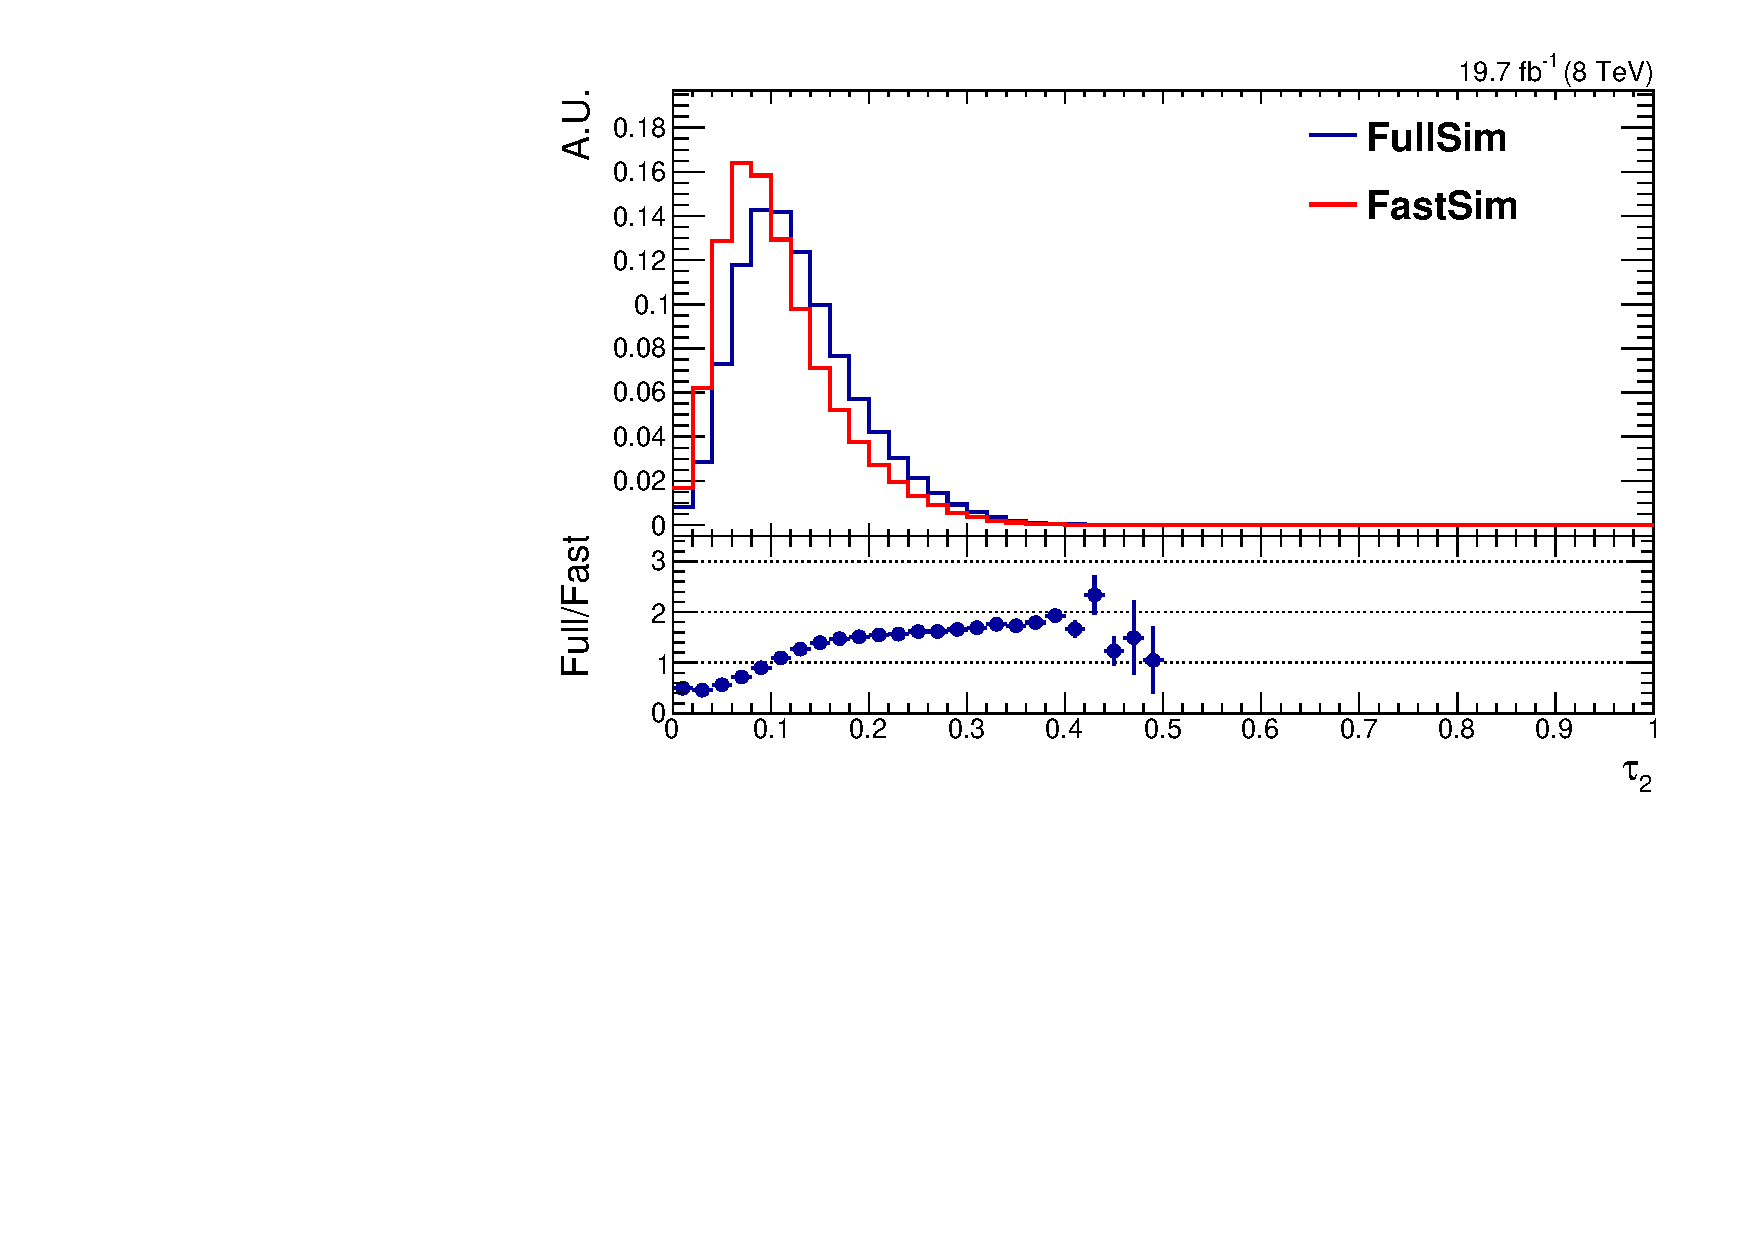
\includegraphics[width=0.49\textwidth]{figures/SF_Wtag_FullFast/FastFull_comparison_TTJets_tau2}
% 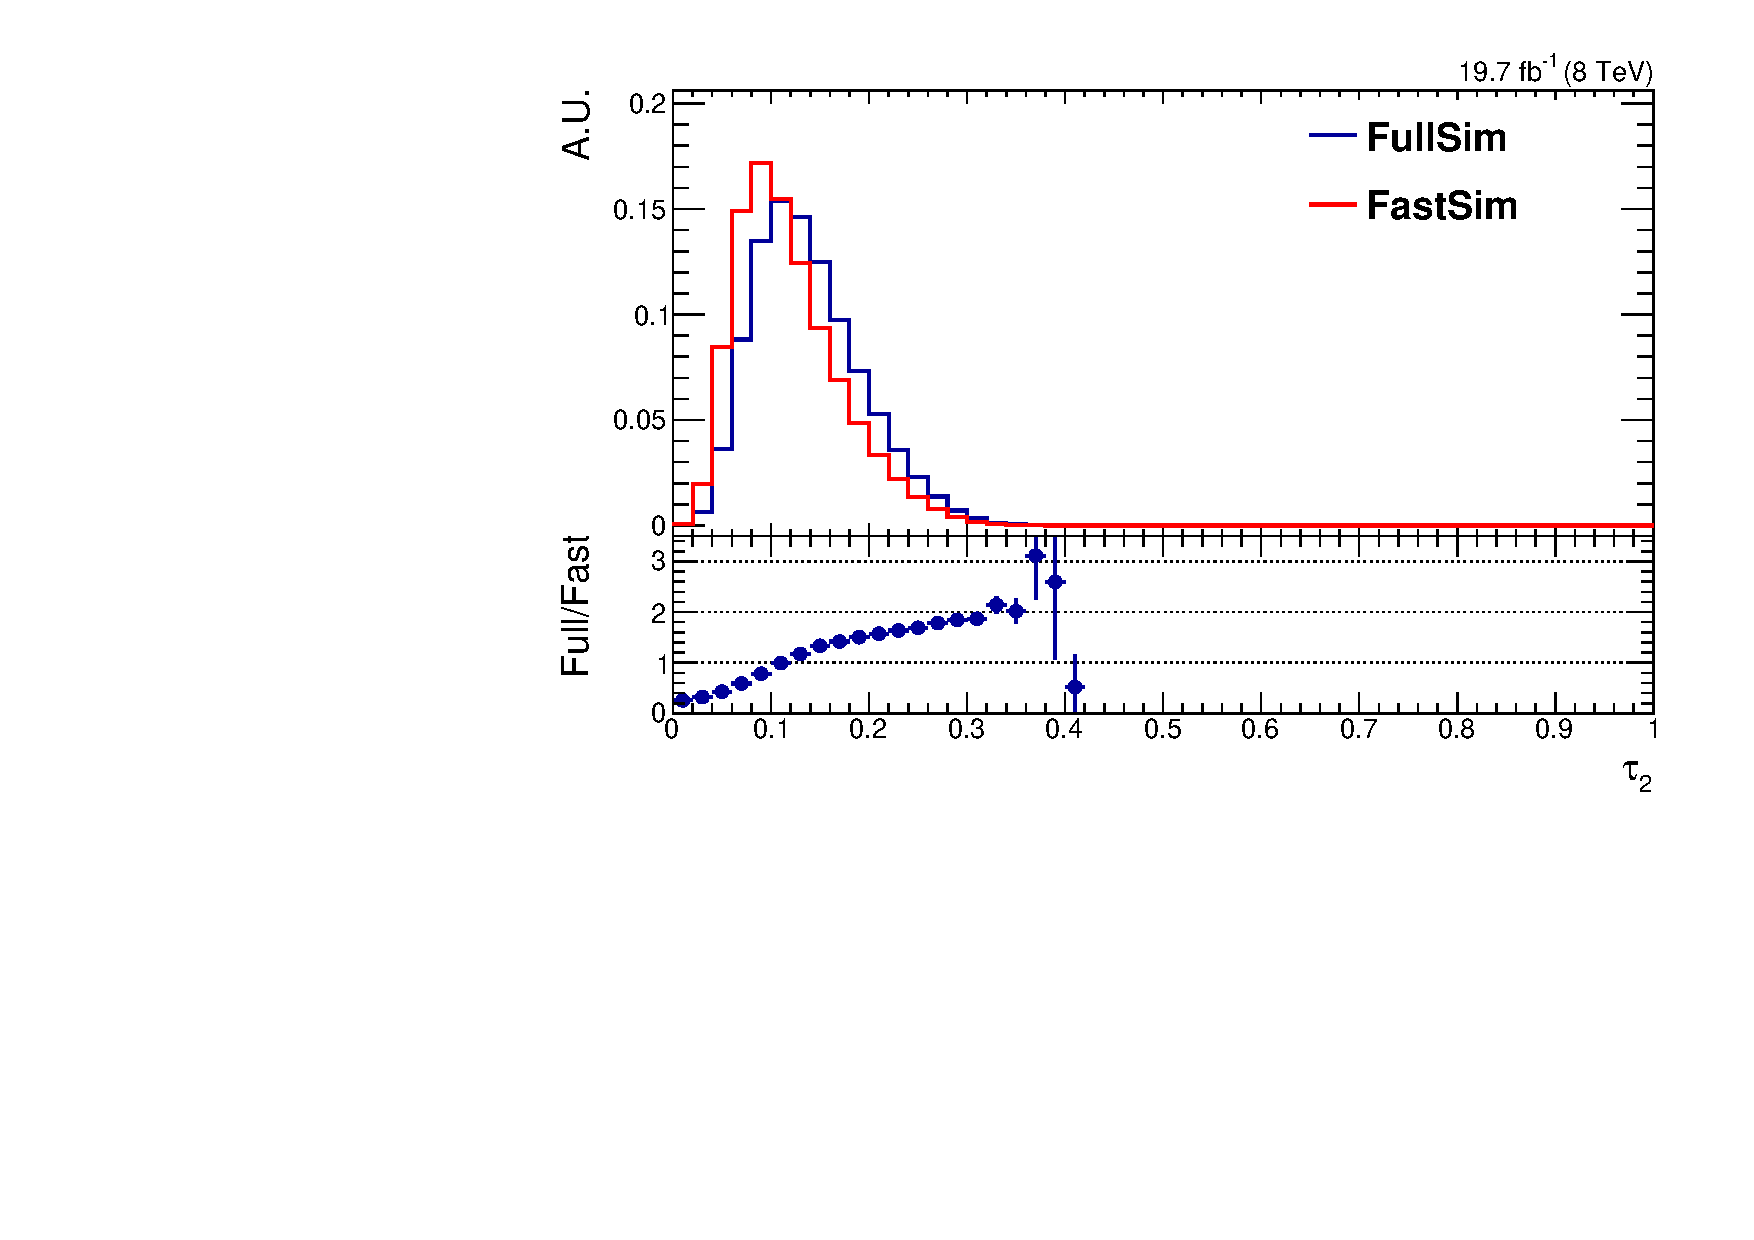
\includegraphics[width=0.49\textwidth]{
% figures/SF_Wtag_FullFast/FastFull_comparison_TTJets_tau2_masscut}
% \caption{Distribution of $\tau_2$ before (left) and after (right) requiring $70 <
% m_{\textrm{jet}}^{\textrm{pruned}} < 100$\GeV, for FastSim and FullSim $t\bar{t}$.
% \label{fig:FastFull_tau2}}
% \end{figure}
% 
% \begin{figure}[p]
% 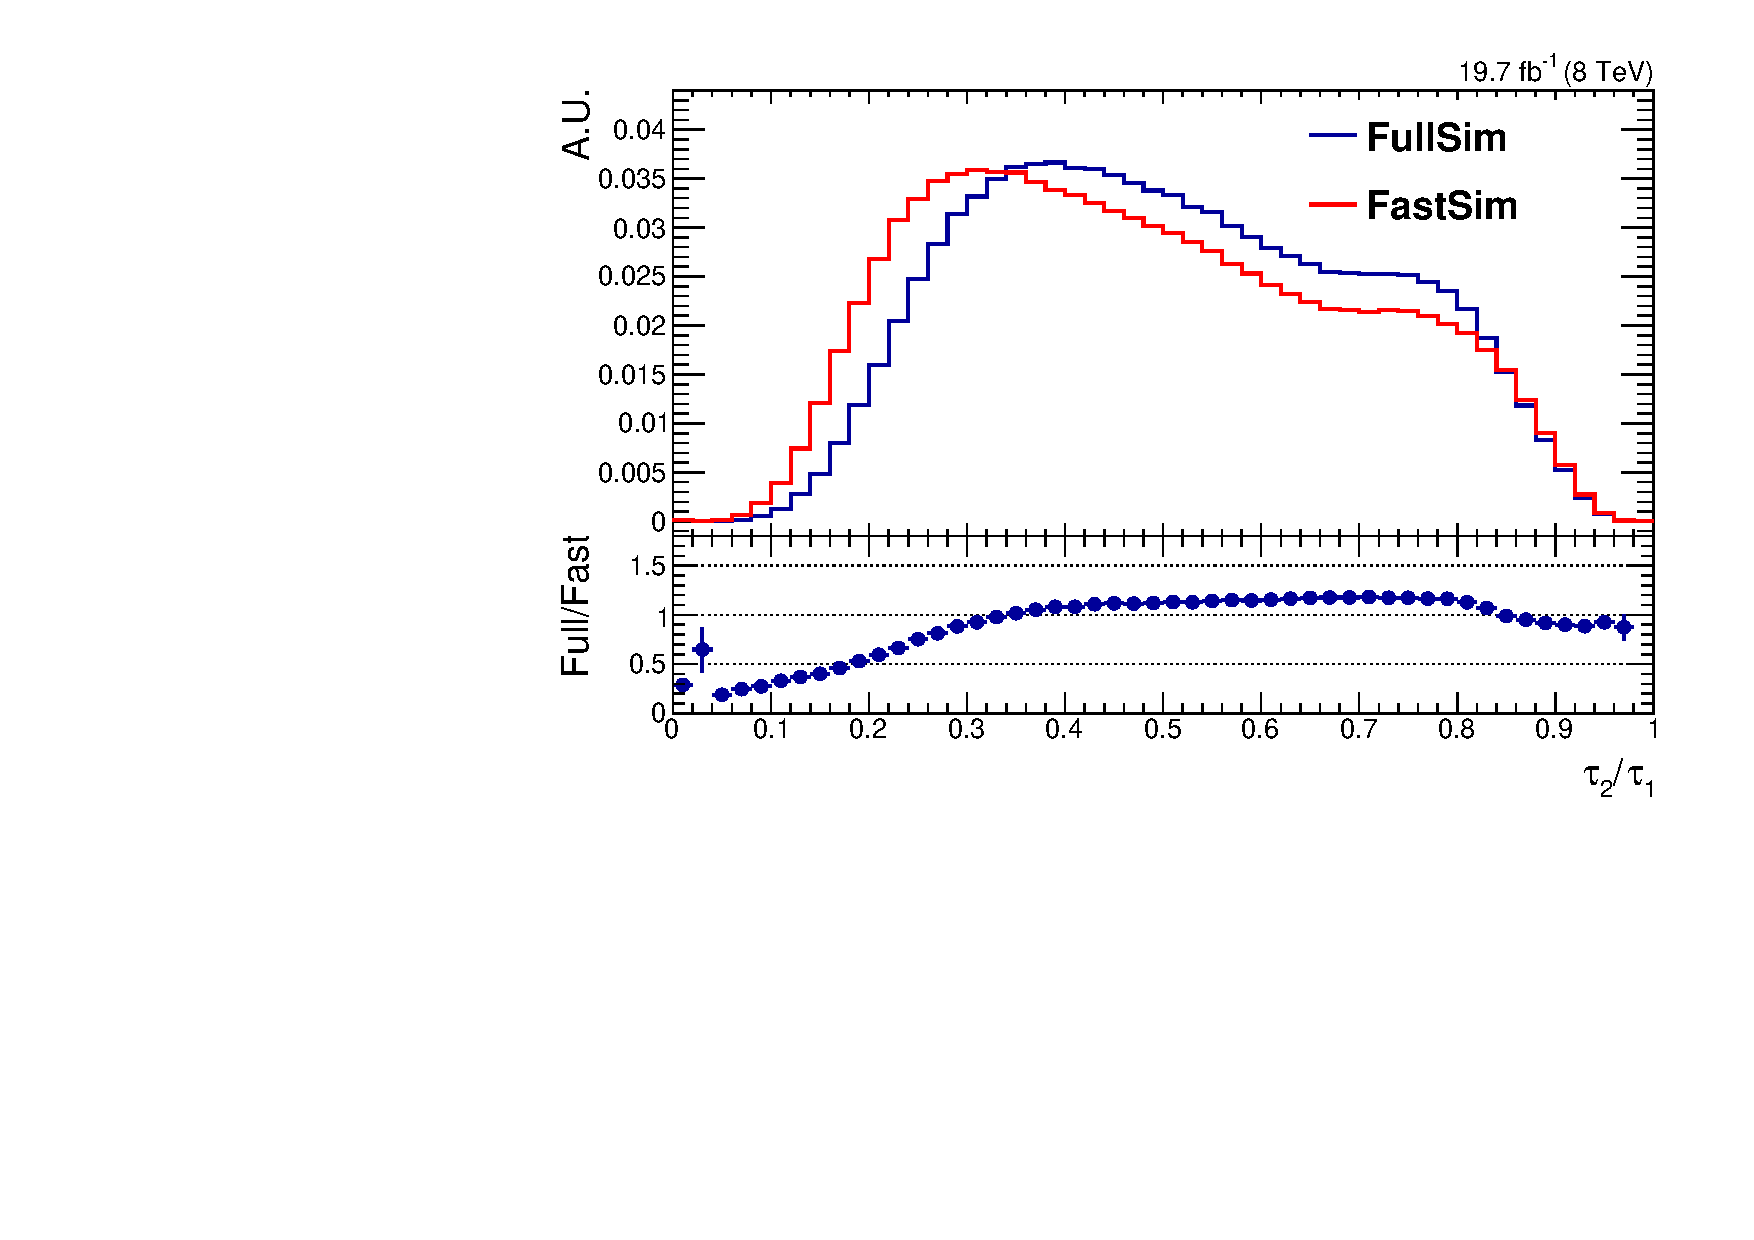
\includegraphics[width=0.49\textwidth]{figures/SF_Wtag_FullFast/FastFull_comparison_TTJets_tau21}
% 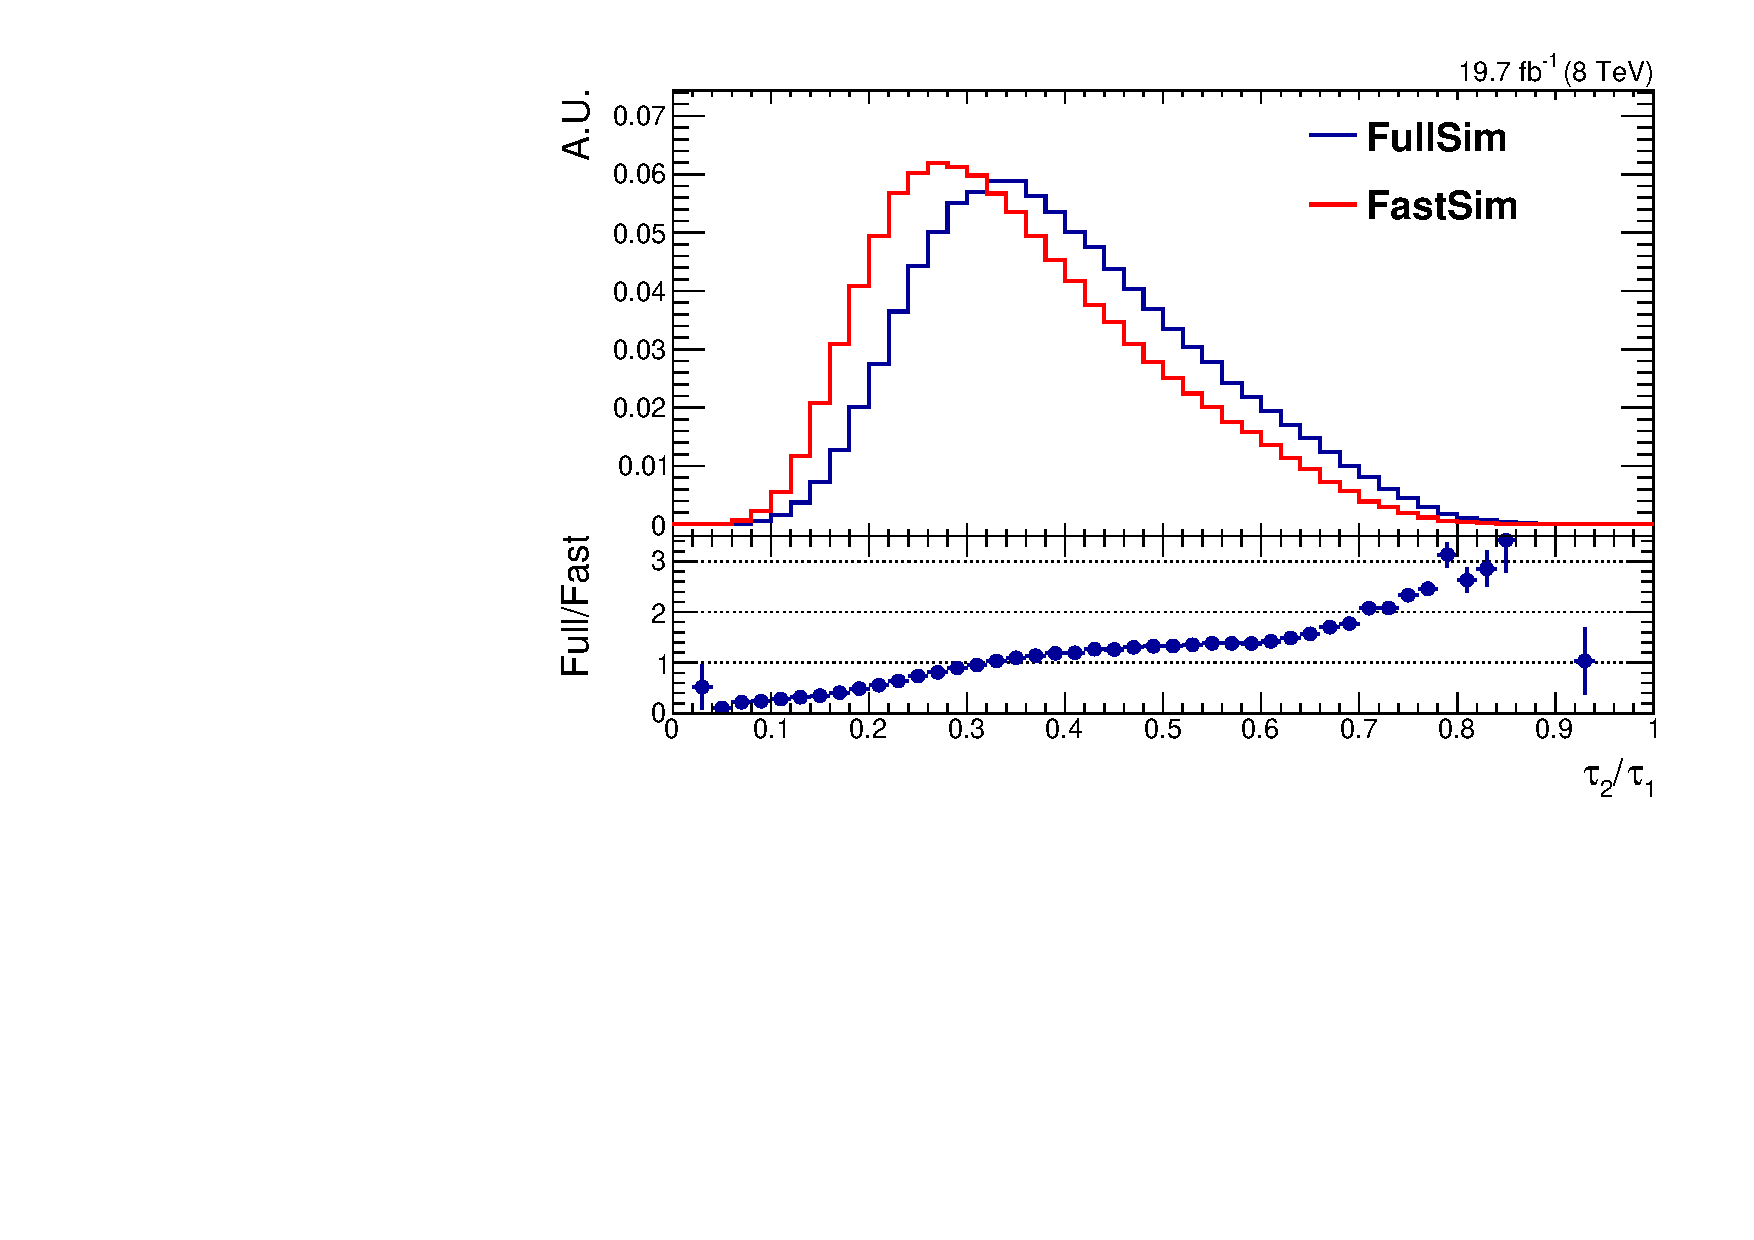
\includegraphics[width=0.49\textwidth]{
% figures/SF_Wtag_FullFast/FastFull_comparison_TTJets_tau21_masscut}
% \caption{Distribution of $\frac{\tau_2}{\tau_1}$ before (left) and after (right) requiring $70 <
% m_{\textrm{jet}}^{\textrm{pruned}} < 100$\GeV, for FastSim and FullSim $t\bar{t}$.
% \label{fig:FastFull_tau21}}
% \end{figure}
% 
% We start by determining the $\PW$ tag efficiency for both samples using this procedure: 
% \begin{enumerate}
% \item Filter the events at generator level, requiring exactly one hadronically decaying $\PW$ to be
% present. 
% \item For this $\PW$, find the closest CA8 jet, and require that it is within $\Delta R = 0.8$ from
% the $\PW$. If no such jet exists, do not select the event. 
% \item Require that there is no $\cPqb$ quark from the top decay within the cone of the selected CA8
% jet. (We only want to select boosted $\PW$'s, not boosted tops.)
% \item For the events that pass the above, plot the \pt distribution of the CA8 jet at three
% selection levels:
%  \begin{itemize}
%    \item no additional selection
%    \item $70 < \textrm{jet mass} < 100$ \GeV
%    \item $70 < \textrm{jet mass} < 100$ \GeV and $\tau_{21} < 0.5$
%  \end{itemize}
% \item By dividing those $p_T$ distributions, we can obtain three efficiencies: 
%  \begin{itemize}
%    \item Efficiency for a matched CA8 jet to have a mass within the W mass window
%    \item Efficiency for a matched CA8 jet to be fully tagged, given that it has a mass within the W
% mass window 
%    \item Efficiency for a matched CA8 jet to be fully tagged
%  \end{itemize}
% \end{enumerate}
% 
% These efficiencies are shown, using two different binnings, in Figure~\ref{fig:eff_Full} for FullSim
% and in Figure~\ref{fig:eff_Fast} for FastSim. 
% \begin{figure}[p]
% \includegraphics[width=0.49\textwidth]{figures/SF_Wtag_FullFast/Wtag_eff_Full_ratio_Wmass_all}
% \includegraphics[width=0.49\textwidth]{figures/SF_Wtag_FullFast/Wtag_eff_Full_ratio_Wmass_all_varbin
% }
% 
% \includegraphics[width=0.49\textwidth]{figures/SF_Wtag_FullFast/Wtag_eff_Full_ratio_tagged_Wmass}
% \includegraphics[width=0.49\textwidth]{
% figures/SF_Wtag_FullFast/Wtag_eff_Full_ratio_tagged_Wmass_varbin}
% 
% \includegraphics[width=0.49\textwidth]{figures/SF_Wtag_FullFast/Wtag_eff_Full_ratio_tagged_all}
% \includegraphics[width=0.49\textwidth]{
% figures/SF_Wtag_FullFast/Wtag_eff_Full_ratio_tagged_all_varbin}
% 
% \caption{Various W-tagging efficiency plots for TTJets FullSim simulation. Left and right are the
% same plot, just with different binning; 
%          [Top] Efficiency for a matched jet to have a mass within the W window; 
%          [Middle] Efficiency for a matched jet to be fully tagged given that it has a mass within
% the W window;
%          [Bottom] Efficiency for a matched jet to be fully tagged. 
% \label{fig:eff_Full}}
% \end{figure}
% 
% \begin{figure}[p]
% \includegraphics[width=0.49\textwidth]{figures/SF_Wtag_FullFast/Wtag_eff_Fast_ratio_Wmass_all}
% \includegraphics[width=0.49\textwidth]{figures/SF_Wtag_FullFast/Wtag_eff_Fast_ratio_Wmass_all_varbin
% }
% 
% \includegraphics[width=0.49\textwidth]{figures/SF_Wtag_FullFast/Wtag_eff_Fast_ratio_tagged_Wmass}
% \includegraphics[width=0.49\textwidth]{
% figures/SF_Wtag_FullFast/Wtag_eff_Fast_ratio_tagged_Wmass_varbin}
% 
% \includegraphics[width=0.49\textwidth]{figures/SF_Wtag_FullFast/Wtag_eff_Fast_ratio_tagged_all}
% \includegraphics[width=0.49\textwidth]{
% figures/SF_Wtag_FullFast/Wtag_eff_Fast_ratio_tagged_all_varbin}
% 
% \caption{Various W-tagging efficiency plots for the TTJets fast simulation. Left and right are the
% same plot, just with different binning; 
%          [Top] Efficiency for a matched jet to have a mass within the W window; 
%          [Middle] Efficiency for a matched jet to be fully tagged given that it has a mass within
% the W window;
%          [Bottom] Efficiency for a matched jet to be fully tagged
% \label{fig:eff_Fast}}
% \end{figure}
% 
% To determine the FullSim/FastSim scalefactor, we use the binning as shown in the right-hand plots of
% figures~\ref{fig:eff_Full} and \ref{fig:eff_Fast}. 
% The scale factor is given by: 
% \begin{equation}
% SF(\pt) = \frac{\epsilon_{FullSim}(\pt)}{\epsilon_{FastSim}(\pt)}
% \end{equation}
% The scale factor as a function of the $p_T$ of the W-candidate is shown in
% figure~\ref{fig:SF_FullFast} and listed bin by bin in table~\ref{tab:SF_FullFast}. 
% 
% \begin{figure}[p]
% \centering
% \includegraphics[width=0.49\textwidth]{figures/SF_Wtag_FullFast/Wtag_SF_FastFullSF_Wmass}
% \includegraphics[width=0.49\textwidth]{figures/SF_Wtag_FullFast/Wtag_SF_FastFullSF_Wmass_varbin}
% 
% \includegraphics[width=0.49\textwidth]{figures/SF_Wtag_FullFast/Wtag_SF_FastFullSF_tagged}
% \includegraphics[width=0.49\textwidth]{figures/SF_Wtag_FullFast/Wtag_SF_FastFullSF_tagged_varbin}
% 
% \caption{[Top] FullSim/FastSim scalefactor for the efficiency for a matched CA8 jet to have a mass
% within the W window; 
%          [Bottom] FullSim/FastSim scalefactor for W-tagging efficiency}
% \label{fig:SF_FullFast}
% \end{figure}
% 
% \begin{table}[htpb]
% \centering
% \caption{Summary of FullSim/FastSim scale factor for W-tagging efficiency}
% \vspace{1ex}
% \begin{tabular}{| c | c | c |}
% \hline
% $p_T$ range & Scale factor & Statistical uncertainty \\
% \hline
% 200-250 &  0.952  &  0.010 \\
% 250-350 &  0.912  &  0.012 \\
% 350-Inf &  0.891  &  0.026 \\
% \hline
% \end{tabular}
% \label{tab:SF_FullFast}
% \end{table}
